\documentclass[mathserif,handout]{beamer}
%\documentclass{beamer}
\usetheme{metropolis}
\usepackage{amsmath,verbatim}
\usepackage{listings}
\usepackage[english]{babel}
%\usepackage{movie15}
\setbeamercovered{transparent}

\newcommand{\Deltap}{\ensuremath{\Delta^{\!+}}}
\newcommand{\trans}{\ensuremath{{}^\mathrm{T}}}
\newcommand{\eps}{\varepsilon}
\newcommand*{\approxdist}{\mathrel{\vcenter{\offinterlineskip
\vskip-.25ex\hbox{\hskip.55ex$\cdot$}\vskip-.25ex\hbox{$\sim$}
\vskip-.5ex\hbox{\hskip.55ex$\cdot$}}}}

% \lstMakeShortInline[language=myR]¬

\lstdefinelanguage{myR}
{
   language=R,
   otherkeywords={read.table, set.seed, head},
   deletekeywords={url,codes, t, dt, Call, formula,Q, R, on,by,hat,is,
col, set,start,end,deltat,zip},
   sensitive=true,
   breaklines=true,
   morecomment=[l]{\#},
   morestring=[b]",
   morestring=[b]',
   basicstyle =\ttfamily\small,
   keywordstyle=\bfseries,
   showtabs=false,
   showstringspaces=false,
   literate= {~}{$\sim$}{2},
   numberstyle=\sffamily\scriptsize,
   stepnumber=2
 }



\title{Statistical modelling for genome-wide screening experiments}
\author{\textbf{\large Darren 
Wilkinson} \\
\url{@darrenjw}\\
\alert{\url{tinyurl.com/darrenjw}}\\
Newcastle University and The Alan Turing Institute\\}
\date{The Francis Crick Institute, London\\24th January, 2017}

\begin{document}

\frame{\titlepage}

\frame{
  \frametitle{The Alan Turing Institute}
  \begin{itemize}
  \item The UK's national institute for Data Science and AI\\ \alert{\url{www.turing.ac.uk}}
  \item A partnership of 13 UK Universities with relevant expertise
  \item HQ in the British Library --- significant space across Levels 1, 2 and~4 --- admin/visitor space on Level 1
  \item Mix of people who work full-time in the HQ, and hot-desks for part-time staff and visitors
  \item Around 200 Turing Fellows (typically senior academics) who spend part of their time at the Turing
    \item In addition to the University partners, the Turing builds partnerships with other large organisations (eg. GCHQ, Lloyd's Register Foundation, Intel, HSBC, UCLH, ...)
  \end{itemize}
}

\frame{
  \frametitle{Relevant Turing programmes}
  \begin{itemize}
    \item Much of the Turing's activity is organised through 10 research programmes, each led by a Programme Director (PD)
    \item Health --- PD: Chris Holmes (Oxford) - joint with HDR UK
      \begin{itemize}
      \item Broad remit, including underpinning bioscience for health
      \item Large programme --- people taking on specific areas --- eg. ``molecular medicine'' (underpinning mechanisms, DJW)
      \item Forming a partnership with UCLH (Sebastian Vollmer, Warwick), and we would be keen to develop another with The Crick - eg. joint appointments for collaborative projects
      \end{itemize}
    \item Data science for science --- PD: Jon Rowe (Birmingham)
      \begin{itemize}
      \item Broad remit, including fundamental bioscience research
      \item We're currently planning a scoping workshop with a focus on research institutes including the LMB and The Crick: working title: \alert{Advanced statistical modelling and machine learning for molecular biology} --- funding collaborative projects, leveraging SPF funding --- May 2019?
      \end{itemize}
  \end{itemize}
}

\frame{
\frametitle{Overview}
\begin{itemize}
%\item Background: Budding yeast as a model for genetics
\item High-throughput robotic genetic experiments
\item Image analysis and data processing
\item Stochastic modelling of growth curves
\item Hierarchical modelling of genetic interaction
\item Bayesian inference for a network of genetic interactions
%\item Functional approaches to scalable Bayesian modelling
%\item Potential CDT PhD project
%\item ``Big data'' challenges, summary and conclusions
\end{itemize}

Joint work with \alert{Jonathan Heydari}, \alert{Keith Newman}, \alert{Conor Lawless} and \alert{David Lydall} (and
others in the ``Lydall lab'')
\bigskip

Major funders: \alert{BBSRC}, \alert{MRC}, \alert{Wellcome Trust}, \alert{CRUK}

}



\section{Yeast}

\subsection{Budding yeast biology and genetics}

\frame{
\frametitle{Saccharomyces cerevisiae}
\begin{itemize}
\item \emph{Saccharomyces cerevisiae}, often known as budding yeast,
and sometimes as brewer's yeast or baker's yeast, is a single-celled
\alert{eukaryotic} organism
\item Eukaryotic cells contain a nucleus (and typically other
organelles, such as mitochondria)
%\item Budding yeast is an interesting species commercially, due to its use in
%baking, beer brewing, wine making, yeast extract, etc.
\item It is useful as a model for higher eukaryotes, having a
great deal of biological function \alert{conserved with humans}
\item It is the most heavily studied and well-characterised
model organism in biology (eg. first fully sequenced eukaryote)
\end{itemize}
}

\begin{comment}
  
\frame{
\frametitle{Budding yeast under the microscope}
\centerline{\includegraphics[height=0.9\textheight]{figs/S_cerevisiae_under_DIC_microscopy}}
}

\end{comment}

\subsection{Synthetic genetic array}

\frame{
\frametitle{Synthetic Genetic Array (SGA)}
\begin{itemize}
\item Possible to obtain a \alert{library} of around 4,500 
%MATa (haploid) 
mutant strains, each of which has one of the non-essential genes 
silenced through insertion of a (kanMX) antibiotic resistance 
cassette and tagged with a unique DNA barcode
\item These strains (stored frozen in 96-well plates) can be
manipulated by robots in 96-well plates (8$\times$12), or on solid
agar in 96, 384 or 1536-spot format
\item \alert{Synthetic Genetic Array} (SGA) is a clever genetic procedure
using robots to systematically introduce an additional mutation into
each strain in the library by starting from a specially constructed
%MAT$\alpha$ 
\alert{query strain} containing the new mutation
\end{itemize}
}


\subsection{Telomeres}

\frame{
\frametitle{Telomeres}
\begin{itemize}
\item The ends of linear chromosomes require special protection in
order not to be targeted by DNA damage repair machinery (bacteria
often avoid this problem by having just one chromosome arranged in a
single loop)
%\item The 2009 Nobel Prize for Physiology and Medicine was awarded to
%the discoverers of telomeres and telomerase...
\item \alert{Telomeres} are the ends of the chromosomal DNA (which have a
special sequence), bound with special telomere-capping proteins that
protect the telomeres
\item \alert{CDC13} is an essential \alert{telomere-capping protein} in yeast
\item \emph{cdc13-1} is a point-mutation of
\emph{cdc13}, encoding a \alert{temperature-sensitive} protein which functions similarly to
wild-type CDC13 below around $25\,^{\circ}\mathrm{C}$, and leads to
``telomere-uncapping'' above this temperature
\end{itemize}
}
  
\frame{
\frametitle{Telomeres, ageing and cancer}

Telomere function is critically important to human health,
affecting ageing, cancer, and other diseases. The main
function of telomeres is to stop the ends of chromosomes
initiating the \alert{DNA Damage Response} (DDR), which normally
responds to intra-chromosomal lesions such as \alert{Double Strand
Breaks} (DSBs). In most human somatic cells insufficient
telomerase is expressed to maintain telomere length and
with continuing cell division. Short
telomeres stimulate \alert{cell cycle arrest} (senescence) or
apoptosis and these processes contribute to \alert{ageing}. Another
consequence of telomere failure is \alert{genetic instability} and
\alert{cancer}, induced when telomeres are ``repaired" as if they were
intra-chromosomal DSBs leading to chromosome fusions and
breakage fusion bridge cycles.

}

\section{Experiments}

\subsection{Lydall lab}

\frame{
\frametitle{Yeast Lab}
\begin{itemize}
\item \alert{David Lydall}'s (budding) yeast lab uses a range of high throughput (HTP) technologies for \alert{genome-wide screening} for
interactions relevant to DNA damage response and repair pathways, with
a particular emphasis on telomere maintenance
\item Much of this work centres around the use of \alert{robotic protocols}
in conjunction with genome-wide knockout libraries and \alert{synthetic
genetic array} (SGA) technology to screen for
\alert{genetic interactions} with known telomere maintenance genes 
\item \alert{Quantitative fitness analysis} (QFA) is the term we use for our
  system of robotic image capture, data handling, image analysis and
  data modelling
%(another talk...)
%\item The Lydall lab also utilises microarrays for studying cellular
%responses at the RNA level
%\item Time course HTP data is most useful for making inferences about
%dynamics
%\item \alert{Time course microarray data} is a typical example
\end{itemize}
}


\subsection{HTP yeast SGA robotic screens}

\frame{
\frametitle{Basic structure of an experiment}
\begin{enumerate}
\item Introduce a \alert{mutation} (such as
\emph{cdc13-1}) into an SGA query strain, and then use SGA technology
(and a robot) to \alert{cross} this strain with the single deletion library in
order to obtain a new library of double mutants
\item \alert{Inoculate} the strains into liquid media, grow up to saturation
then spot back on to solid agar 4 times
\item \alert{Incubate} the 4 different copies at different temperatures
(treatments), and image the plates multiple times to see how quickly
the different strains are growing
\item Repeat steps 2 and 3 four times (to get some idea of experimental
variation)
%\item Repeat steps 1 to 4 using a different version of the library
%which has the strains arranged differently on the plates (to
%ameliorate spatial location effects)
\item Repeat steps 2 to 4 with a ``control'' library that does not
  include the query mutation
\end{enumerate}
}

\frame{
\frametitle{Some numbers relating to an experiment}
\begin{itemize}
\item Initial SGA work (introducing mutations into the query and the
library) takes around \alert{1 month} of calendar time, and several days of
robot time
\item The inoculation, spotting and imaging of the 8 repeats takes
  \alert{1 month} of calendar time, and around 2 weeks of robot time
\item The experiment uses around \alert{\pounds 3,000} of consumables
(plastics and media) 
\item The library is distributed across 72 96-well plates or 18 solid agar
plates (in 384 format, or 1536 in quadruplicate)
\item If each plate is imaged 30 times, there will be around 35k
high-resolution photographs of plates in 384 format, corresponding to
around \alert{13 million} colony growth measurements (400k time
series)
\item This is \alert{big data}!
\end{itemize}
}



\frame{
\frametitle{HTP SGA robotic facility}
\centerline{
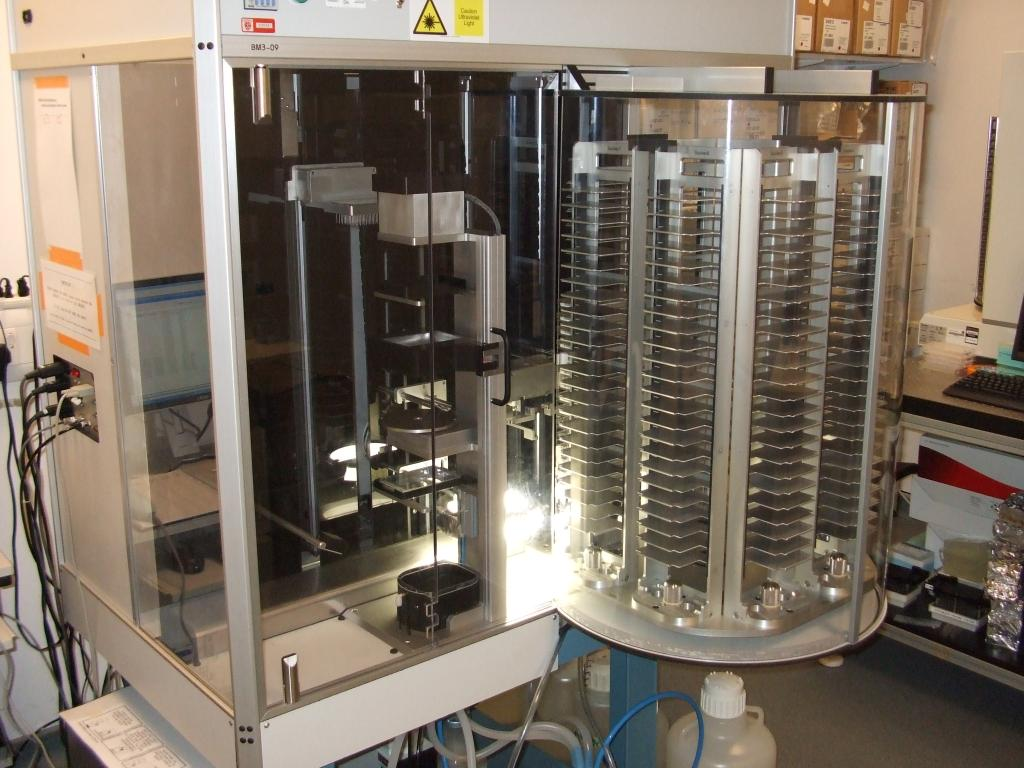
\includegraphics[height=0.4\textheight]{figs/robots-sticky}~
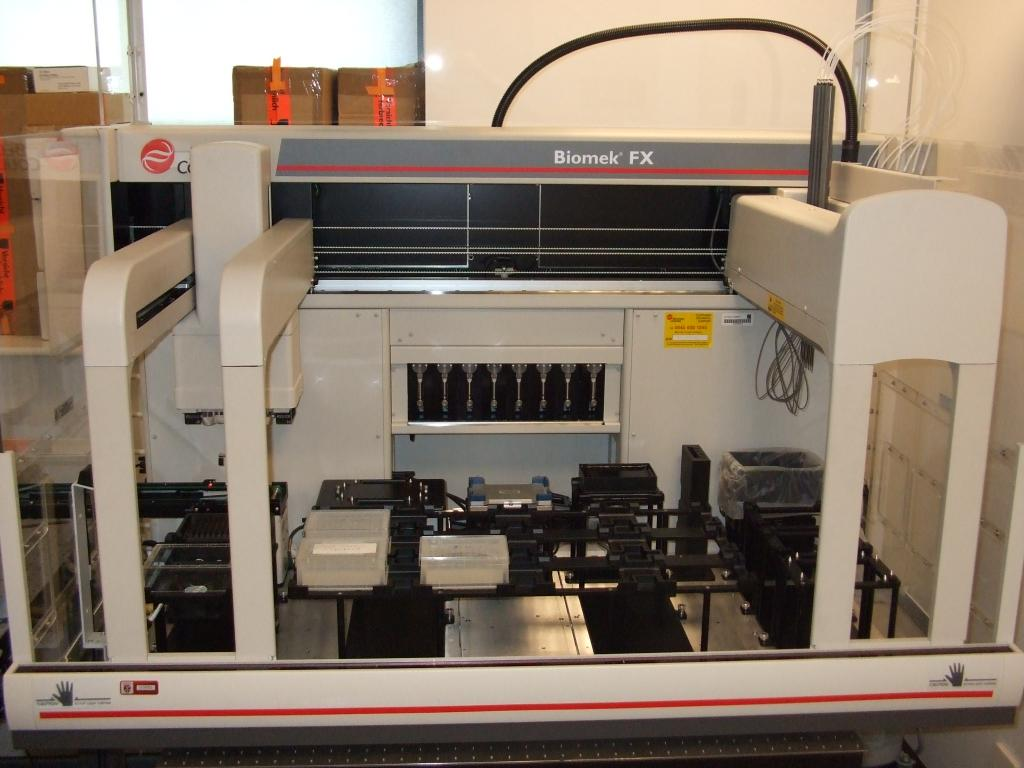
\includegraphics[height=0.4\textheight]{figs/robots-runny}~
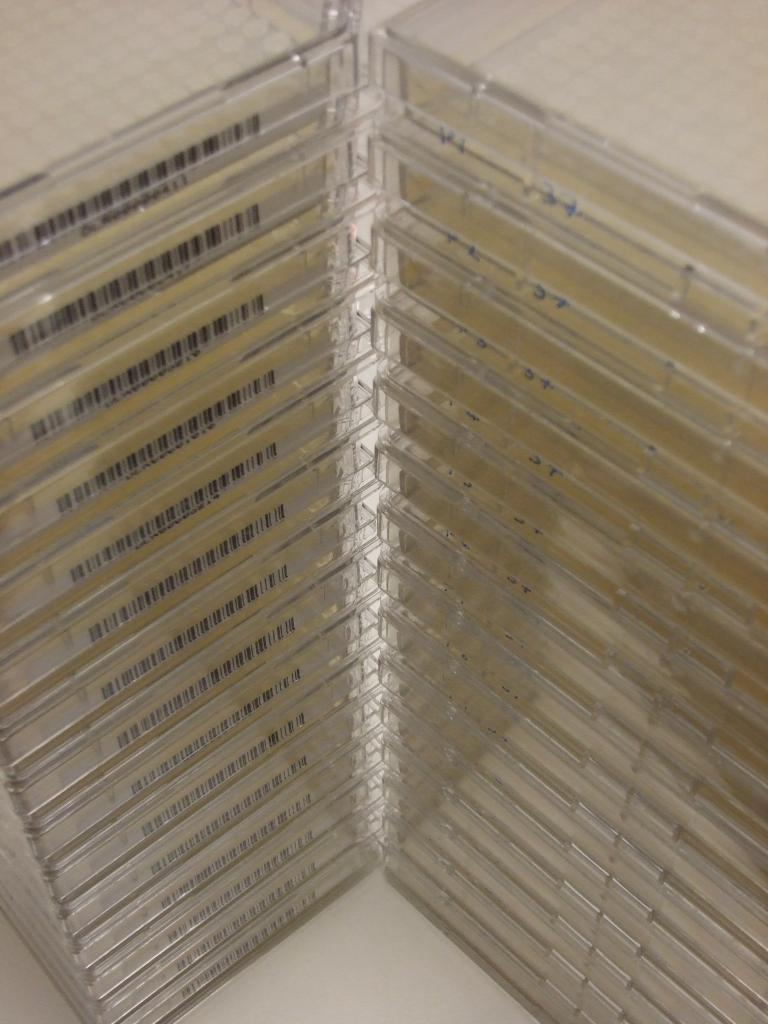
\includegraphics[height=0.4\textheight]{figs/robots-plates}
}
\vspace{0.5ex}
\centerline{
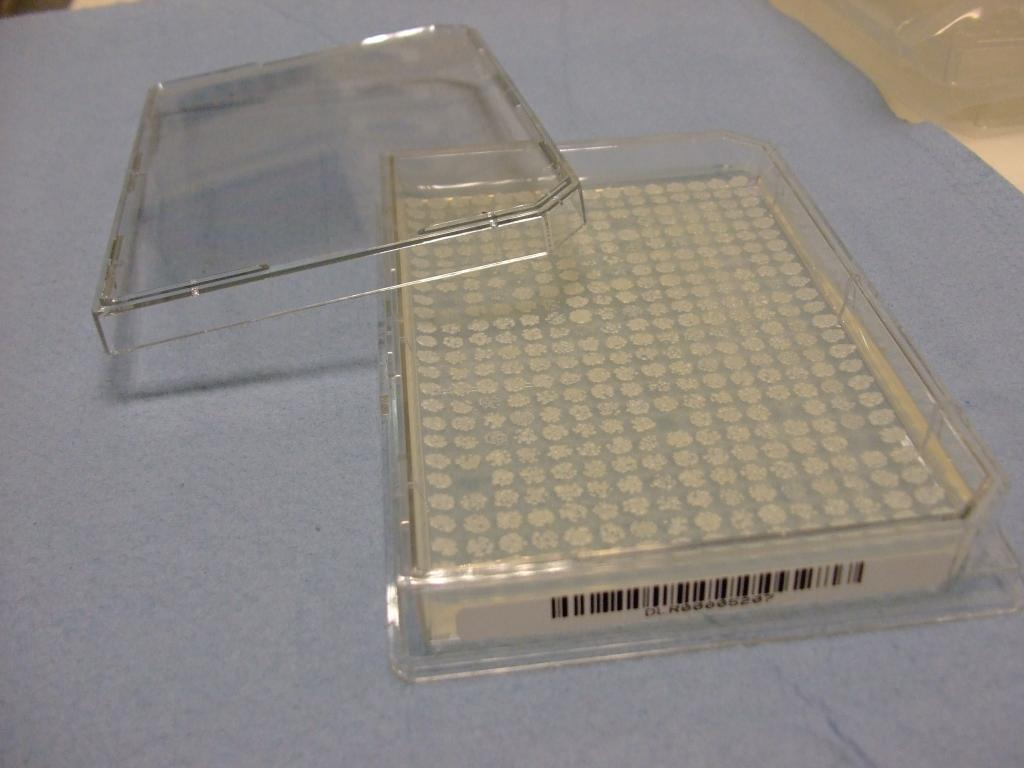
\includegraphics[height=0.4\textheight]{figs/robots-plate}~
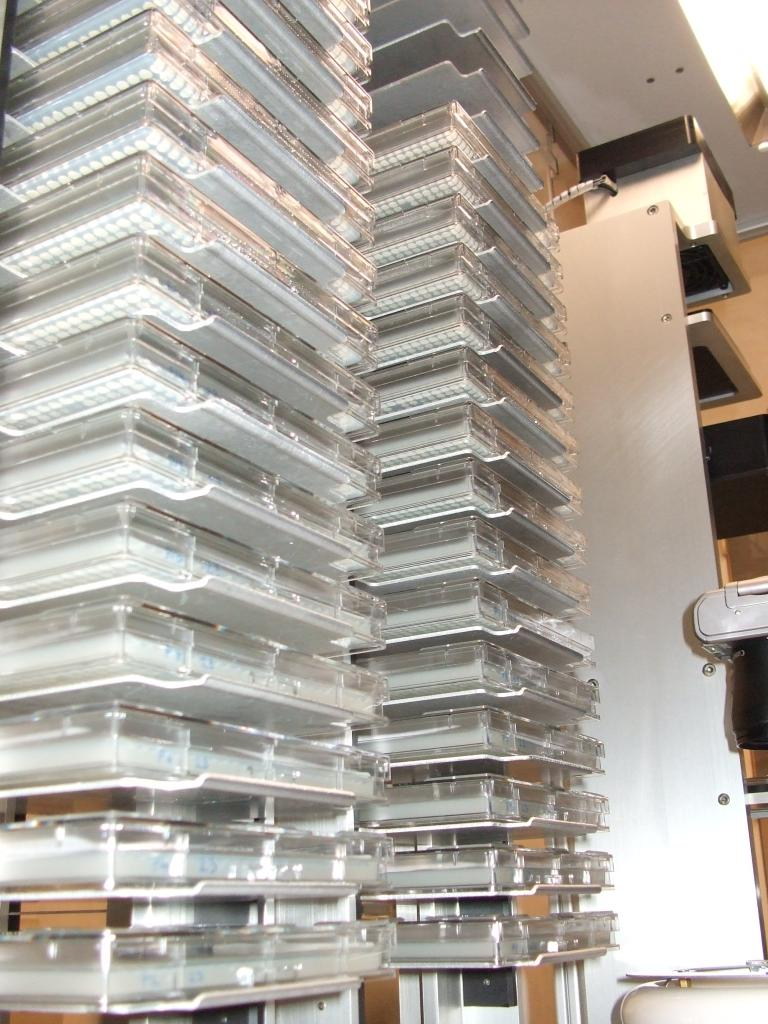
\includegraphics[height=0.4\textheight]{figs/robots-plates-sticky}~
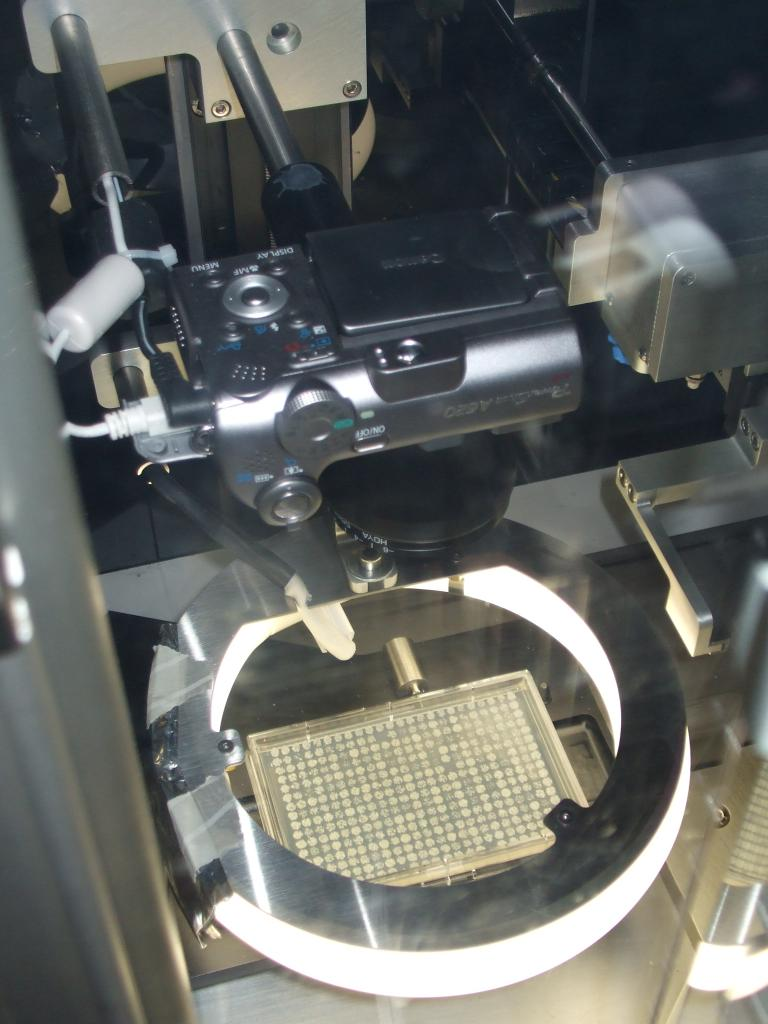
\includegraphics[height=0.4\textheight]{figs/robots-plate-photo}
}
}

\begin{comment}

\frame{
\frametitle{The colony handling robot}
\centerline{\includemovie[poster,text={Loading
movie...}]{0.8\textwidth}{0.8\textheight}{figs/robot.mpg}}
}

\end{comment}


\section{Data analysis}

\subsection{Data analysis pipeline}


\frame{
\frametitle{Data analysis pipeline}
\begin{itemize}
\item \alert{Image processing} (from images to colony size
  measurements)
\item \alert{Fitness modelling} (from colony size growth curves to
  strain fitness measures)
\item \alert{Modelling genetic interaction} (from strain fitness
  measures to identification of genetically interacting strains, ranked
  by effect size)
\end{itemize}
Possible to carry out three stages separately, but benefits to joint
modelling through borrowed strength and proper propagation of
uncertainty. Not practical to integrate image processing step into the
joint model, but possible to jointly model second two stages.
}


%\subsection{Image analysis}

\frame{
\frametitle{Automated image analysis (Colonyzer)}
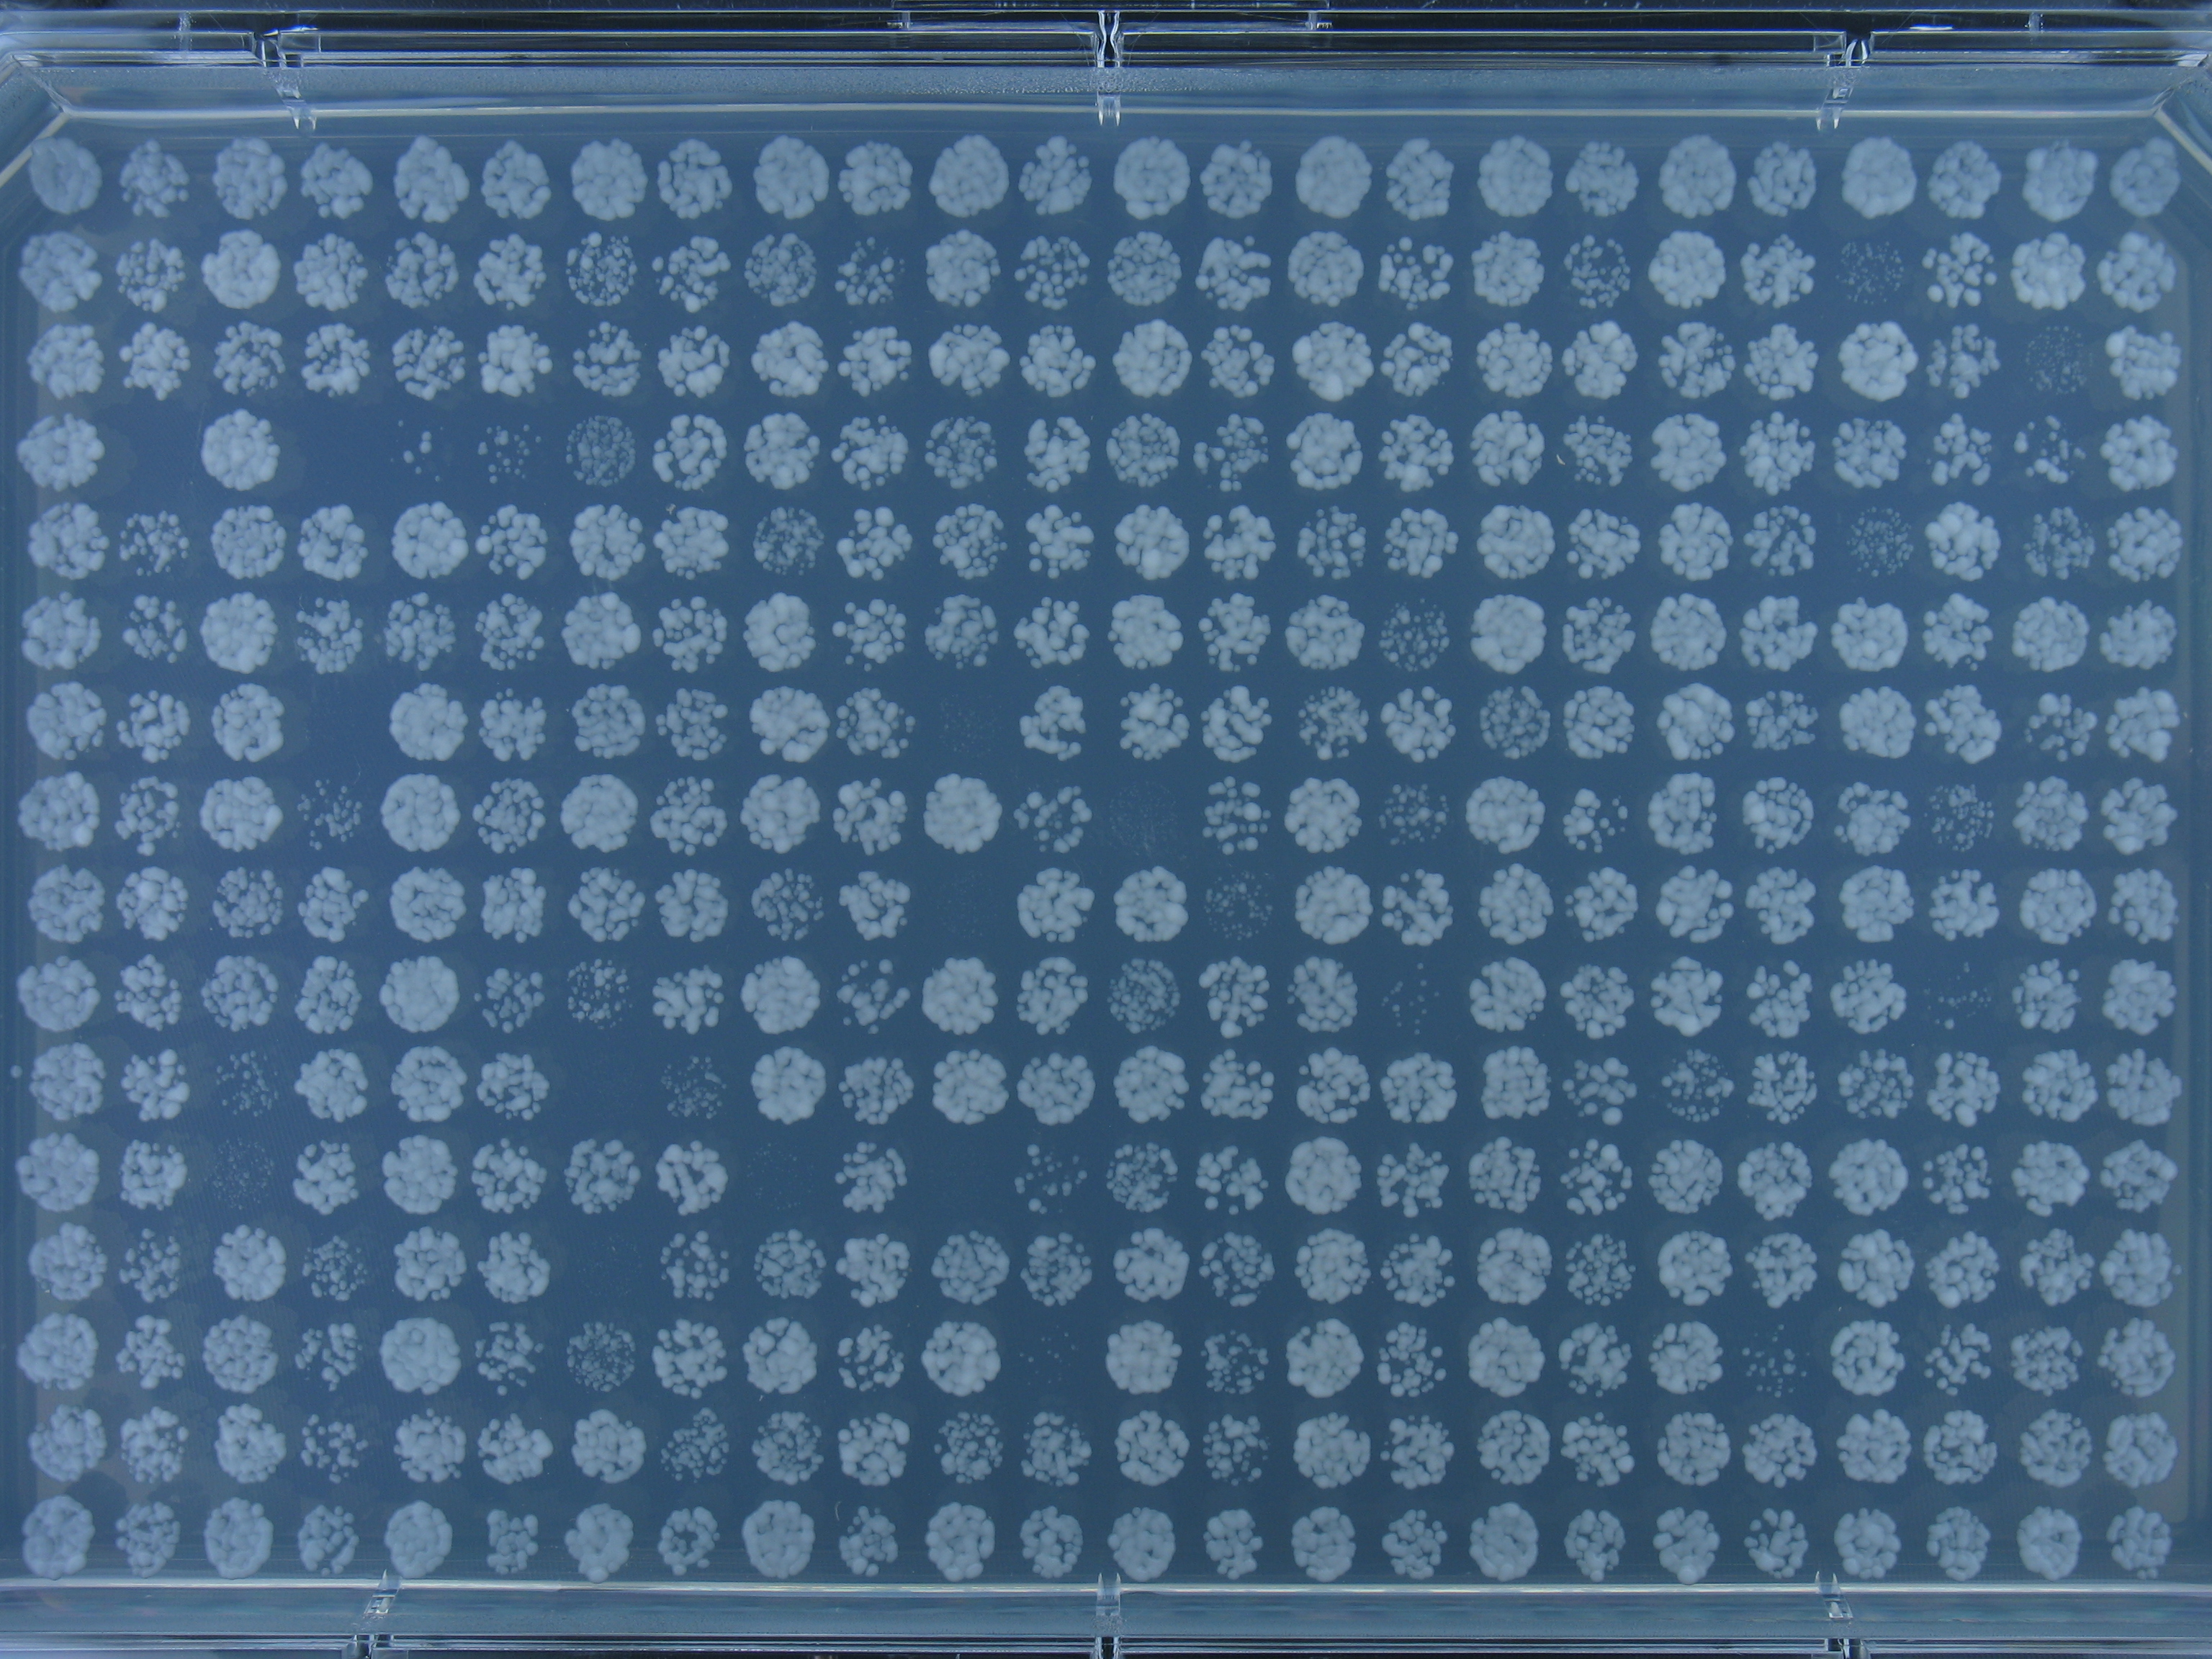
\includegraphics[height=0.38\textheight]{figs/rod-plate}\hspace{3ex}
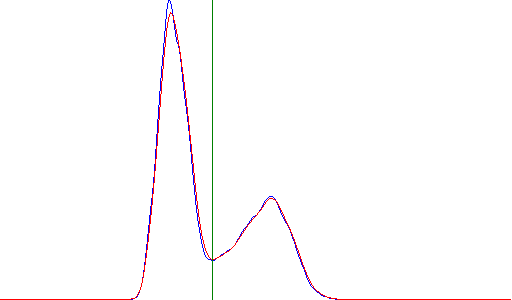
\includegraphics[height=0.38\textheight]{figs/rod-plate-hist}
\vspace{1ex}\\
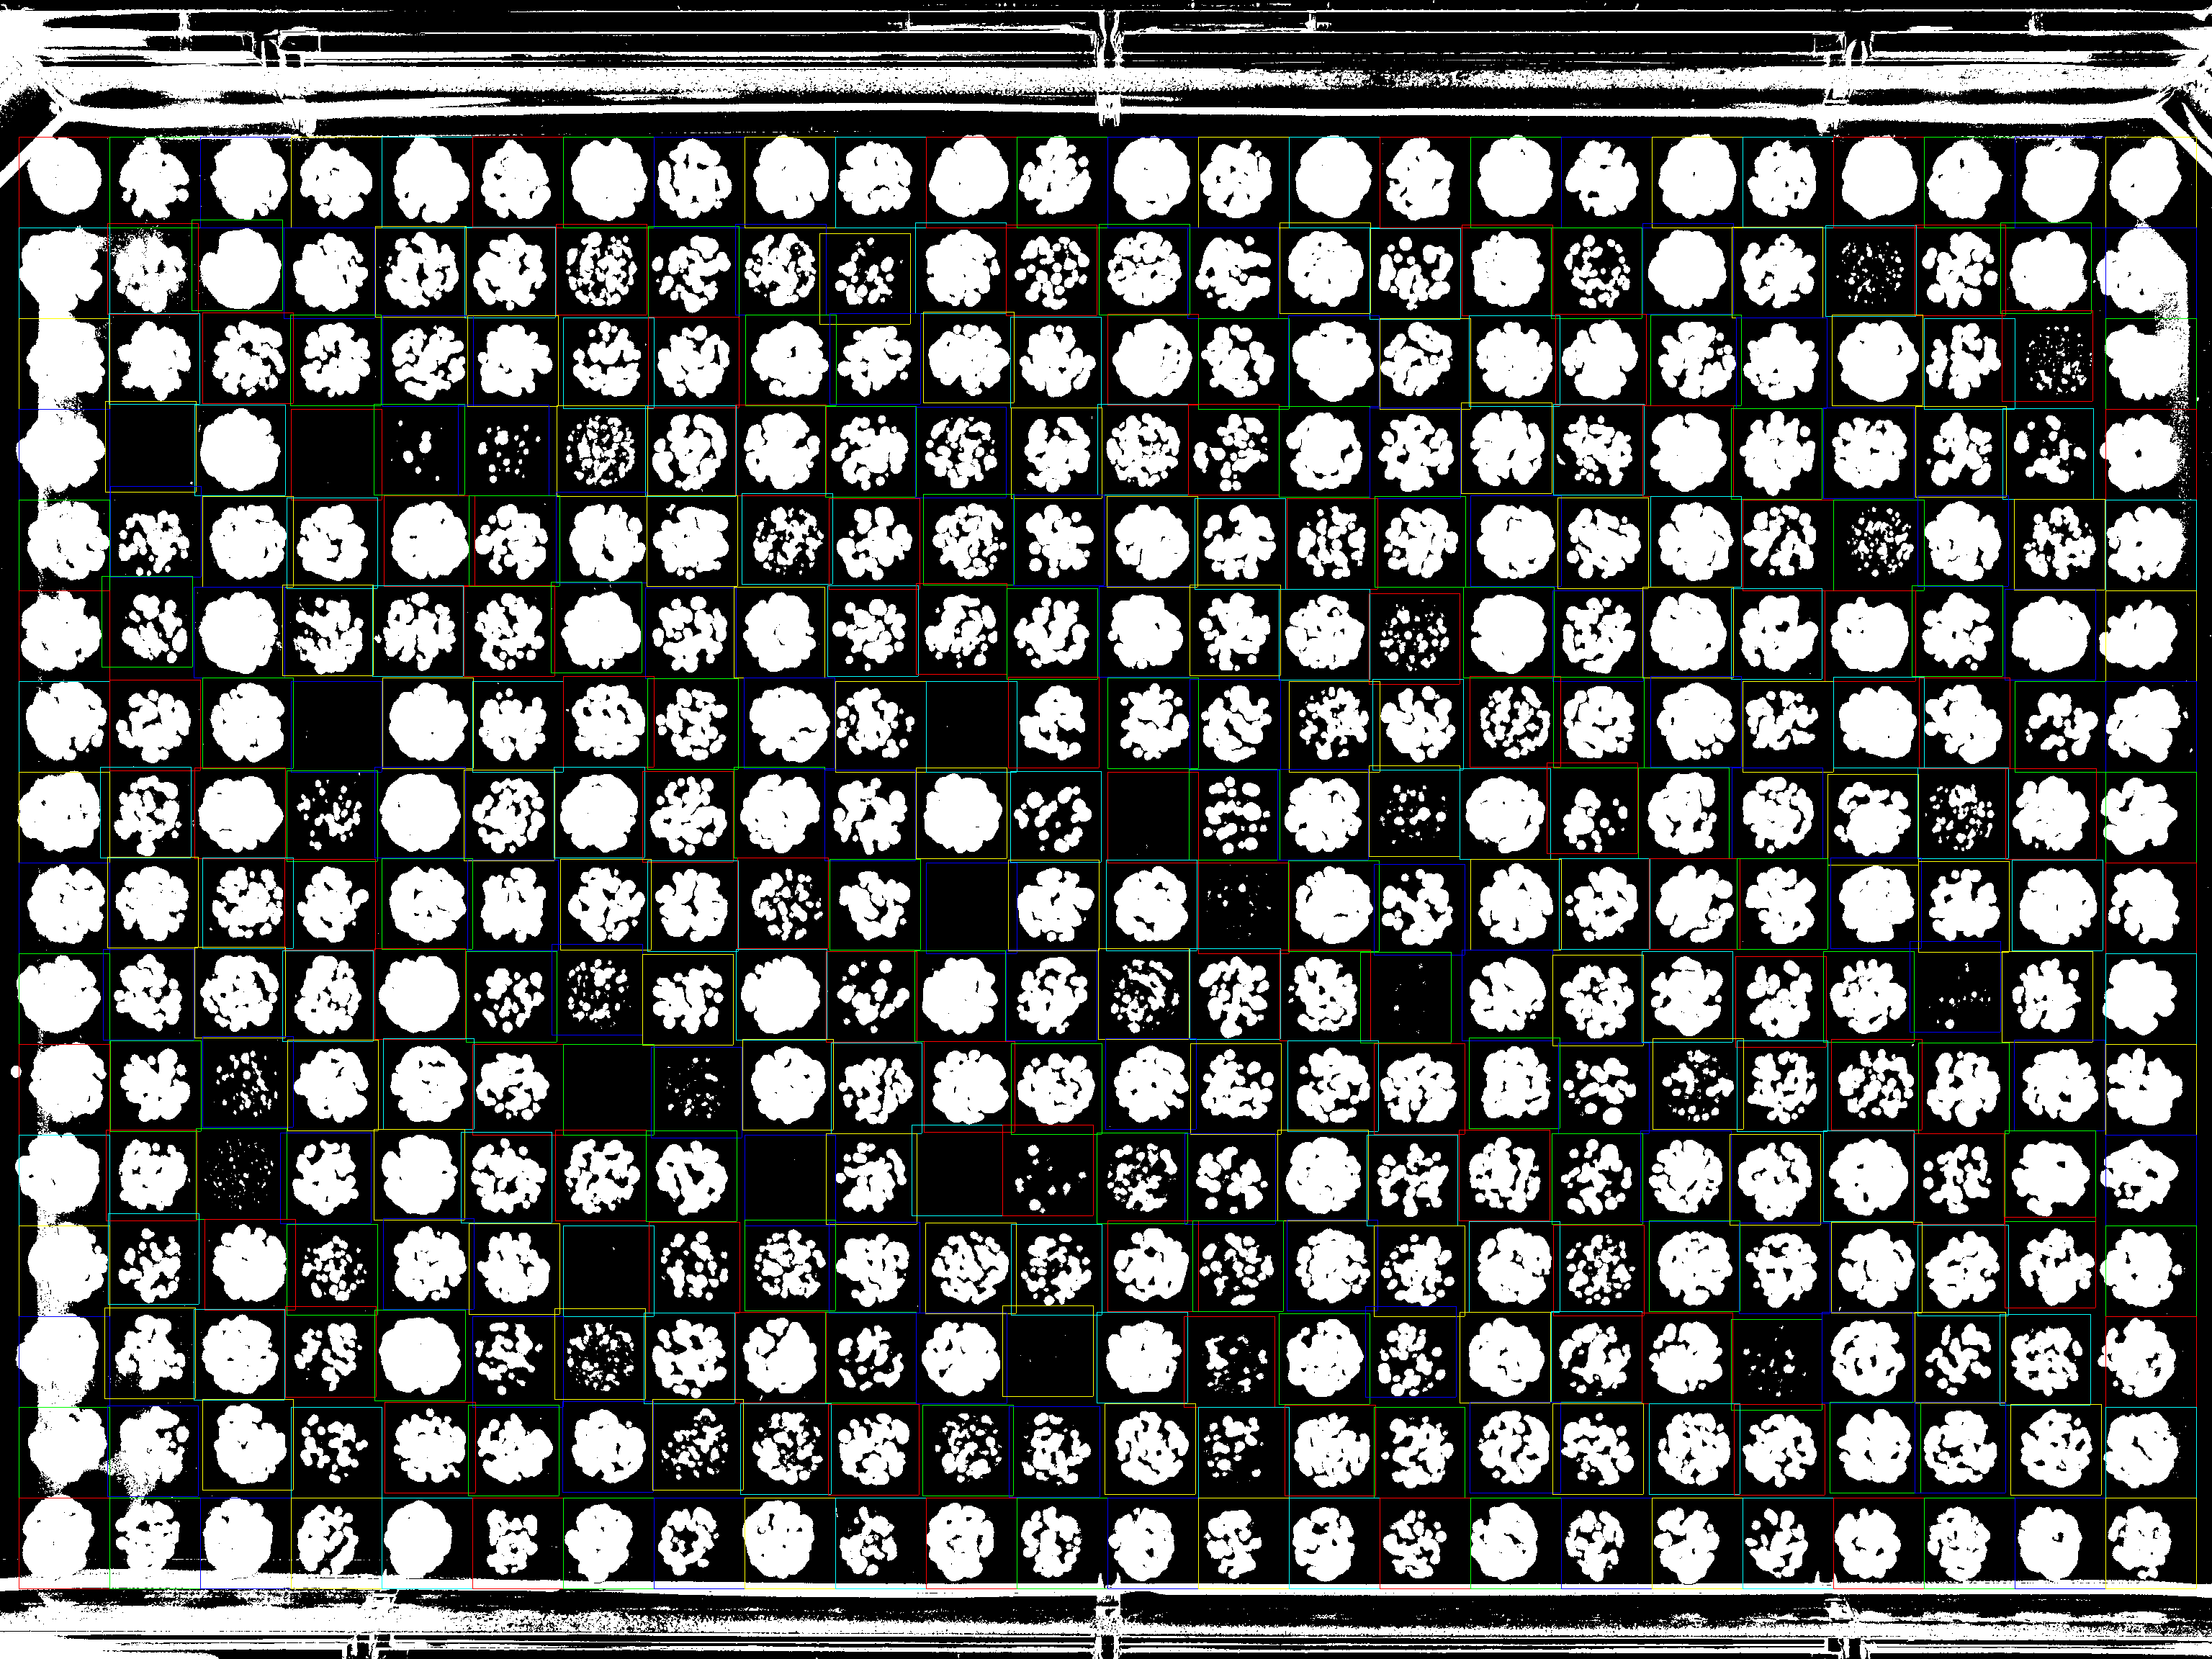
\includegraphics[height=0.38\textheight]{figs/rod-plate-grid-thresh}\hspace{8ex}
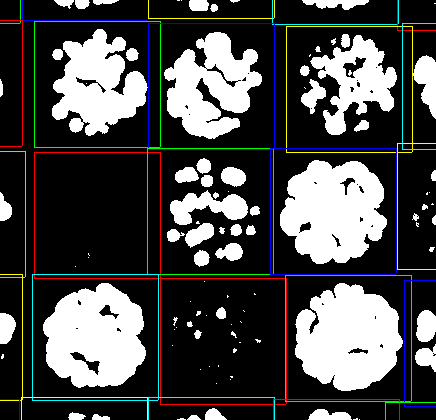
\includegraphics[height=0.38\textheight]{figs/rod-plate-grid-thresh-zoom}

}


\subsection{Growth curve modelling}

\frame{
\frametitle{Growth curve}
\centerline{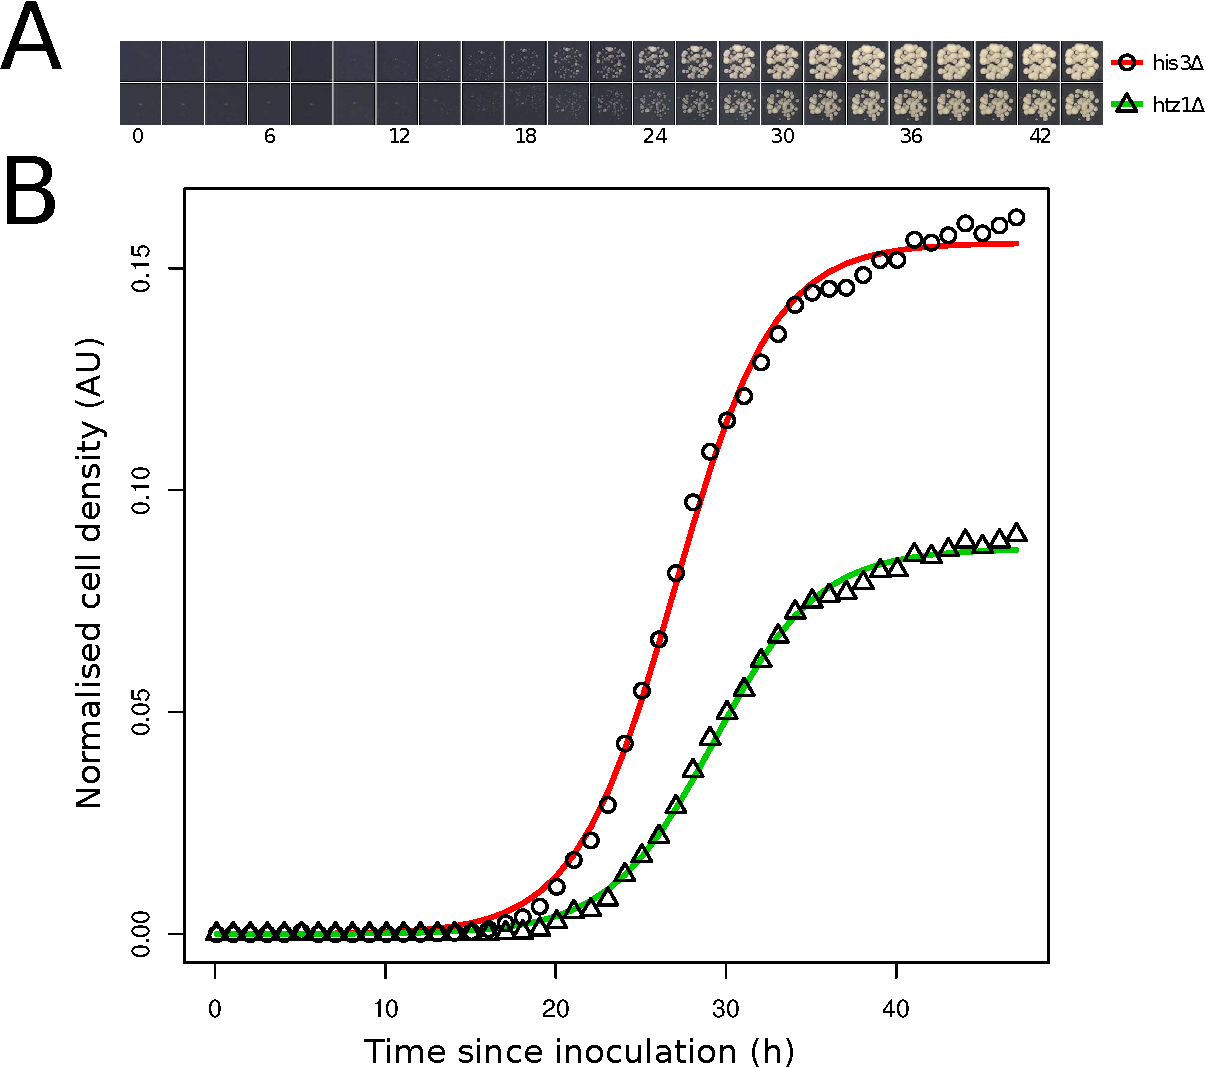
\includegraphics[height=0.8\textheight]{figs/LawlessfigAB}}
%\centerline{\includegraphics[height=0.8\textheight]{figs/ygc1}}
}

\frame{
\frametitle{Growth curve modelling}
\begin{itemize}
\item We want something between a simple smoothing of the data and a
  detailed model of yeast cell growth and division
\item \alert{Logistic growth models} are ideal --- simple
  semi-mechanistic models with interpretable parameters related to
  strain fitness
\item Basic deterministic model:
\[
\frac{dx}{dt} = rx(1-x/K),
\]
subject to initial condition $x=P$ at $t=0$
\item $r$ is the \alert{growth rate} and $K$ is the \alert{carrying capacity}
\item Analytic solution:
\[
x(t) = \frac{KPe^{rt}}{K+P(e^{rt}-1)}
\]
\end{itemize}
}

\frame{
\frametitle{Statistical model}
\begin{itemize}
\item Model observational measurements $\{Y_{t_1},Y_{t_2},\ldots\}$ with
\[
Y_{t_i} = x_{t_i} + \eps_{t_i}
\]
\item Can fit to observed data $y_{t_i}$ using non-linear least
  squares or MCMC
\item Can \alert{fit all (400k) time courses simultaneously} in a large hierarchical
  model which effectively borrows strength, especially across repeats,
  but also across genes
\item Generally works well (fine for most of the downstream scientific
  applications), but fit is often far from perfect...

\end{itemize}
}


\frame{
\frametitle{Fitting the logistic curve}
\centerline{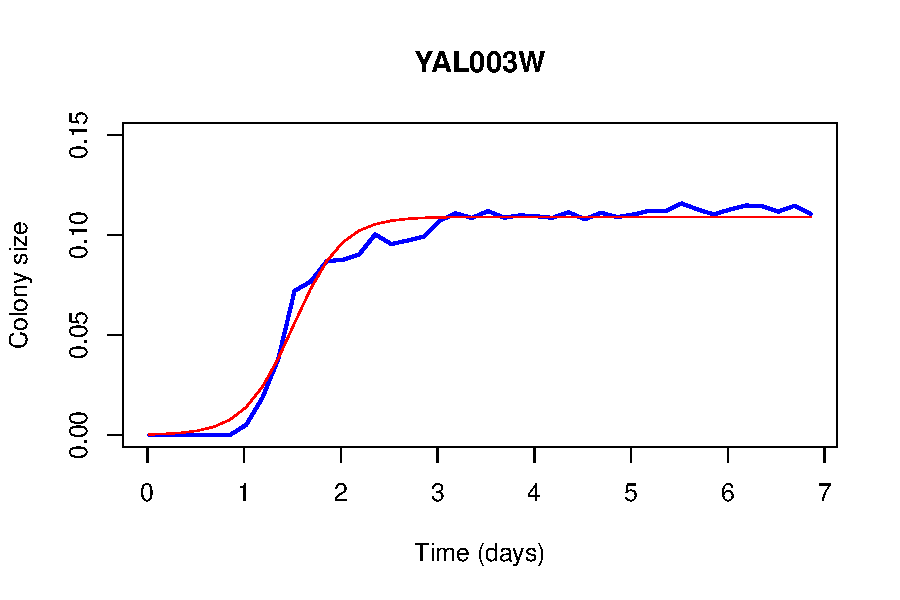
\includegraphics[height=0.8\textheight]{figs/ygc2}}
%Show a bad fit...
}

\frame{
\frametitle{Improved modelling of colony growth curves}
\begin{itemize}
\item Could use a \alert{generalised logistic model} (Richards' 
curve) which
  breaks the symmetry in the shape of ``take off'' and ``landing''
\[
\frac{dx}{dt} = rx(1-(x/K)^\nu)
\]
\item This
  helps, but doesn't address the real problem of strongly
  auto-correlated residuals
\item Better to introduce noise into the dynamics to get a logistic
  growth diffusion process
\end{itemize}
}

\frame{
\frametitle{Stochastic logistic growth diffusion}
\begin{itemize}
\item
Well-known stochastic generalisation of the logistic growth equation,
expressed as an It\^o stochastic differential equation (SDE):
\[
dX_t = rX_t(1-X_t/K)dt + \xi^{-1/2}X_t\,dW_t
\]
\item The \alert{drift} is exactly as for the deterministic model
\item The \alert{diffusion} term injects some noise into the dynamics
\item The \alert{multiplicative noise} ensures that this defines a
  non-negative stochastic process
\end{itemize}
}

\frame{
\frametitle{Sample trajectories from the logistic diffusion}
%\includegraphics[width=0.5\textwidth]{figs/ygc1}
\centerline{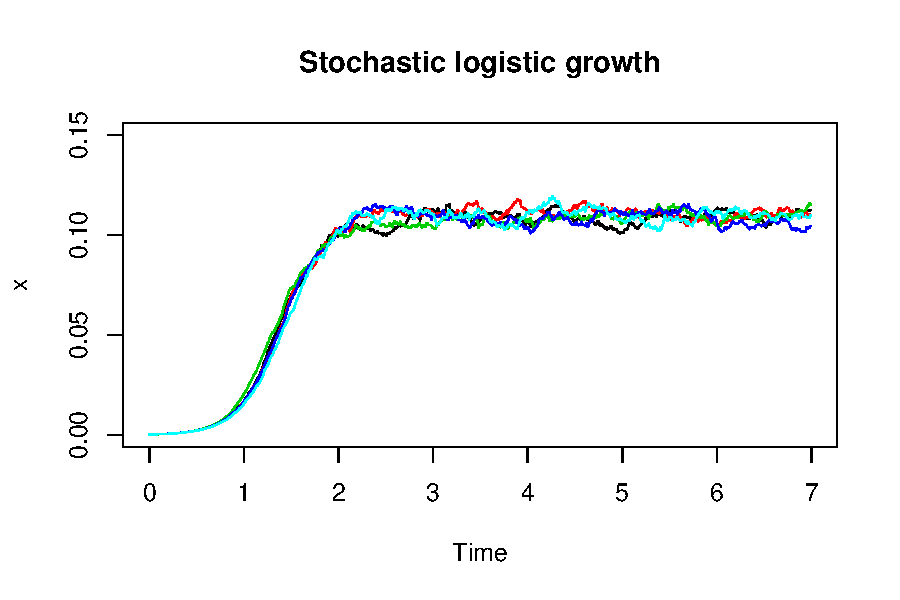
\includegraphics[width=0.8\textwidth]{figs/ygc3}}
}

\frame{
\frametitle{Statistical model}
\begin{itemize}
\item Model observational measurements $\{Y_{t_1},Y_{t_2},\ldots\}$ with
\[
Y_{t_i} = X_{t_i} + \eps_{t_i}
\]
where $X_{t_i}$ refers to our realisation of the diffusion process
\item Need somewhat sophisticated algorithms to fit these sorts of SDE
  models to discrete time data
\item Standard algorithms would require knowledge of the transition
  kernel of the diffusion process, but this is not available for the
  logistic diffusion
\item Lots of work on Bayesian inference for intractable diffusions
  \alert{(Golightly \& W, '05, '06, '08, '10, '11)}, but this won't
  scale to simultaneous fitting of tens of thousands of realisations
\end{itemize}
}

\begin{comment}

\frame{
\frametitle{Approximating the stochastic logistic diffusion}
\begin{itemize}
\item Computational constraints mean that we can only really consider
  working with diffusions having \alert{tractable transition kernels} (as then
  we can apply standard MCMC methods for discrete time problems)
\item If we apply a log transformation to the logistic
  diffusion and then carry out a \alert{linear noise approximation}, the
  result will be a process with log-normal increments
\item Putting $U_t=\log X_t$, It\^o's formula gives
\[
dU_t = \left(r-\frac{1}{2\xi}-\frac{r}{K}e^{U_t}\right)dt + \xi^{-1/2}dW_t
\]
\end{itemize}
}


\frame{
\frametitle{Linear noise approximation (LNA)}
\begin{itemize}
\item Decompose $U_t$ into a deterministic component and a stochastic
  residual process
\[
U_t = v_t + Z_t
\]
where $v_t$ solves the deterministic part
\[
\frac{dv_t}{dt} = r-\frac{1}{2\xi}-\frac{r}{K}e^{v_t}
\]
\item Subtracting out the deterministic solution from $U_t$ leaves a
  residual process of the form
\[
dZ_t = \frac{r}{K}e^{v_t}(1-e^{Z_t})dt+\xi^{-1/2}dW_t
\]
\end{itemize}
}

\frame{
\frametitle{Linear noise approximation (LNA)}
\begin{itemize}
\item Applying the \alert{linear approximation} $1-e^{Z_t}\simeq -Z_t$
  to linearise the drift gives
\[
dZ_t = -\frac{r}{K}e^{v_t}Z_tdt+\xi^{-1/2}dW_t
\]
\item Substituting in for $v_t$ then gives
\[
dZ_t = -\frac{abPe^{at}}{bP(e^{at}-1)+a}Z_tdt+\xi^{-1/2}dW_t,
\]
where $a=r-1/(2\xi)$ and $b=r/K$
\item This is a (zero) mean-reverting time-varying
  \alert{Ornstein--Uhlenbeck} (OU) process, and can
  be solved exactly, giving a normal transition kernel
\end{itemize}
}

\frame{
\frametitle{The logistic diffusion and the LNA}
\includegraphics[width=0.5\textwidth]{figs/ygc4}
\includegraphics[width=0.5\textwidth]{figs/ygc6}

The (log)LNA is a very good approximation to the true process, with
\alert{tractable log-normal increments}
}

\end{comment}

\frame{
\frametitle{Further simplifications and approximations}
\begin{itemize}
\item The \alert{linear noise approximation} (LNA) applied to the log-transformed process is a good model with a tractable transition kernel
\item We can implement standard discrete time MCMC methods to estimate
  model parameters together with the unobserved latent trajectories
\item Embedding in a hierarchical model is straightforward
\item These methods work fine for hundreds of growth curves, but are
  still problematic for tens of thousands of growth curves
\end{itemize}
}

\frame{
\frametitle{Integrating out the latent process}
\begin{itemize}
  \item If we are prepared to assume linear Gaussian error on the log
    scale, we can use \alert{Kalman filtering} techniques to \alert{integrate out} the
    latent process (but this isn't very plausible)
  \item Alternatively, we could apply a LNA directly to the logistic
    diffusion (without first transforming), and assume linear Gaussian
    error on that scale (\alert{Heydari et al, 2013})
  \item This latter approach turns out to be better, despite the fact that the LNA approximation to the true process isn't quite as good
\item More important to have a plausible error structure than a super-accurate approximation to the stochastic process
\end{itemize}
}

\frame{
\frametitle{Growth curve model}
\centerline{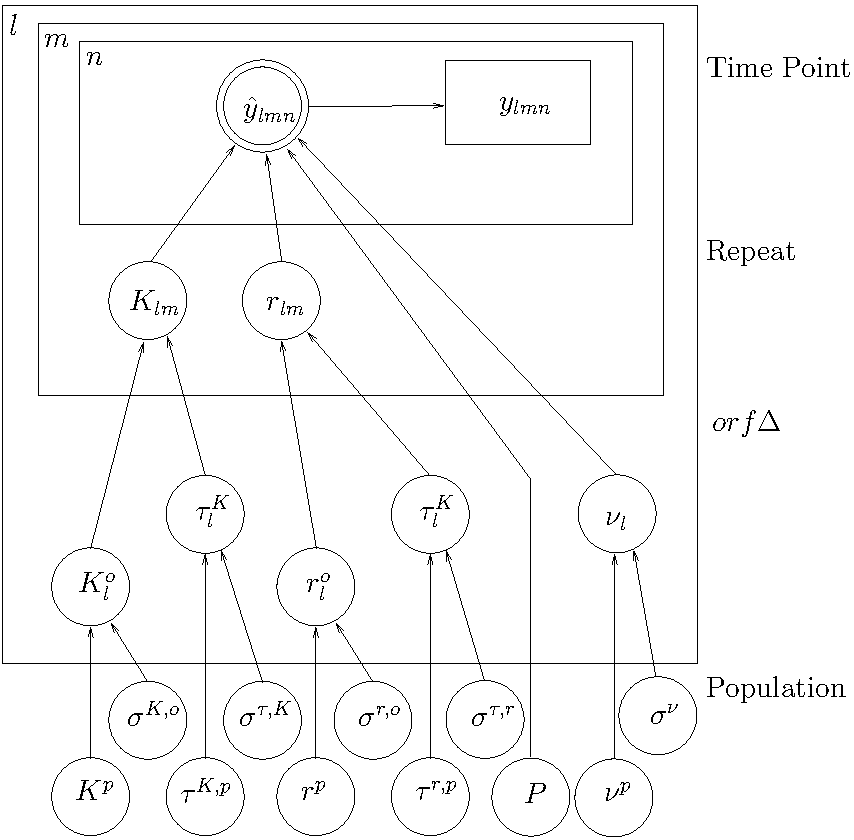
\includegraphics[height=0.8\textheight]{figs/DAG1}}
}

\frame{
\frametitle{Colony fitness}
\begin{itemize}
\item The results of model fitting are estimates (or posterior
  distributions) of $r$ and $K$ for each yeast colony, and also the
  corresponding gene level parameters
\item Both $r$ and $K$ are indicative of colony fitness --- keep
  separate where possible
\item Often useful to have a scalar measure of fitness --- many
  possibilities, including $rK$, $r\log K$, or MDR$\times$MDP, where
  MDR is the
  maximal doubling rate and MDP is the maximal doubling potential
\item Statistical summaries can be fed in as data to the next
  level of analysis (or, ultimately, modelled jointly as a giant
  hierarchical model)
\end{itemize}
}

\subsection{Modelling genetic interaction}

\frame{
\frametitle{Epistasis}
From Wikipedia:
\begin{itemize}
\item \emph{``\alert{Epistasis is the interaction between
genes}. Epistasis takes place when the action of one gene is modified
by one or several other genes, which are sometimes called modifier
genes. The gene whose phenotype is expressed is said to be epistatic,
while the phenotype altered or suppressed is said to be hypostatic.''}
\item \emph{``\alert{Epistasis and genetic interaction refer to the same
phenomenon}; however, epistasis is widely used in population genetics
and refers especially to the statistical properties of the
phenomenon.''}
\end{itemize}
}

\frame{
\frametitle{Multiplicative model}
\begin{itemize}
\item Consider two genes with alleles $a/A$ and $b/B$ with $a$ and
$b$ representing ``wild type'' (note that $A$ and $B$ could potentially
represent knock-outs of $a$ and $b$) 
\item Four genotypes: aa, Ab, aB, AB. Use $[\cdot]$ to denote some
  quantitative phenotypic measure (eg. ``fitness'') for each genotype
\item \alert{Multiplicative model} of genetic independence:
\begin{tabbing}
$[AB]\times [ab] = [Ab]\times [aB]$ \qquad\= no epistasis \\
$[AB]\times [ab] > [Ab]\times [aB]$ \qquad\= synergistic epistasis \\
$[AB]\times [ab] < [Ab]\times [aB]$ \qquad\= antagonistic epistasis 
\end{tabbing}
\item Perhaps simpler if re-written in terms of relative fitness:
\[
\frac{[AB]}{[ab]} = \frac{[Ab]}{[ab]}\times \frac{[aB]}{[ab]}
\]
\end{itemize}
}

\frame{
\frametitle{Genetic independence and HTP data}
\begin{itemize}
\item Suppose that we have scaled our data so that it is
consistent with a multiplicative model --- what do we expect to see?
\item The independence model $[AB]\times [ab] = [Ab]\times [aB]$ translates to
\[
[\text{query}:\text{abc}\Delta] \times [\text{wt}] = [\text{query}] \times
[\text{abc}\Delta]\]
\item In other words
\[
[\text{query}:\text{abc}\Delta]  = \frac{[\text{query}]}{[\text{wt}]} \times
[\text{abc}\Delta]\]
\item That is, the double-mutant differs from the single-deletion by a
constant multiplicative factor that is independent of the particular
single-deletion
\item ie. a scatter-plot of double against single will show them all
lying along a straight line
\end{itemize}
}

\frame{
\frametitle{Statistical modelling}
\begin{itemize}
\item
Assume that $F_{clm}$ is the fitness measurement for repeat $m$ of
gene deletion $l$ in condition $c$ ($c=1$ for the single deletion and
$c=2$ for the corresponding double-mutant)
\item Model:
\begin{align*}
F_{clm} &\sim N(\hat{F}_{cl},1/\nu_{cl}) \\
\log \hat{F}_{cl} &= \alpha_c + Z_l + \delta_l\gamma_{cl} \\
\delta_l &\sim Bern(p)
\end{align*}
\item $\delta_l$ is a variable selection indicator of \alert{genetic
    interaction}
\item Then usual Bayesian hierarchical stuff...
\end{itemize}
}

\frame{
\frametitle{Genetic interaction model}
\centerline{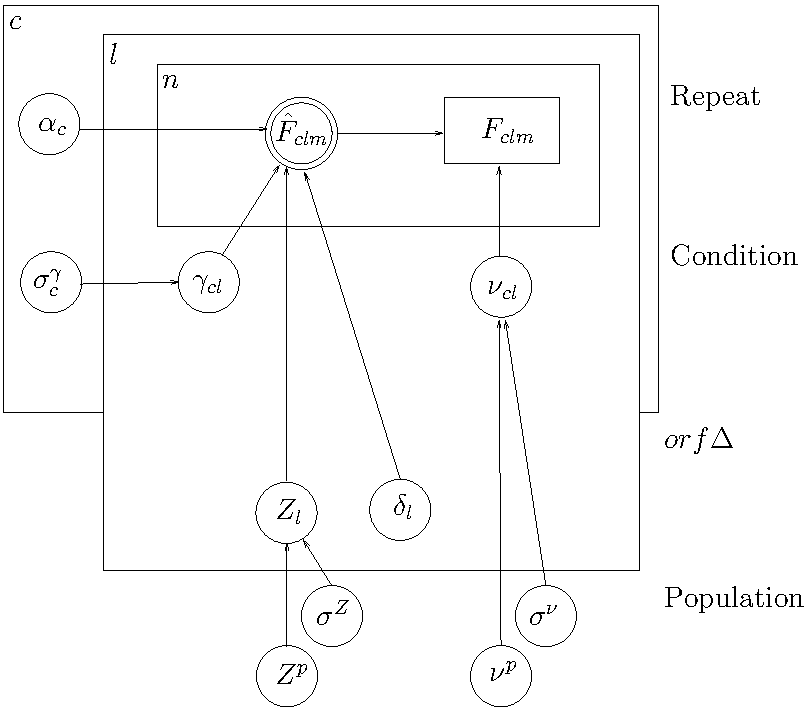
\includegraphics[height=0.8\textheight]{figs/DAG2}}
}

\frame{
\frametitle{Genetic interaction results}
\centerline{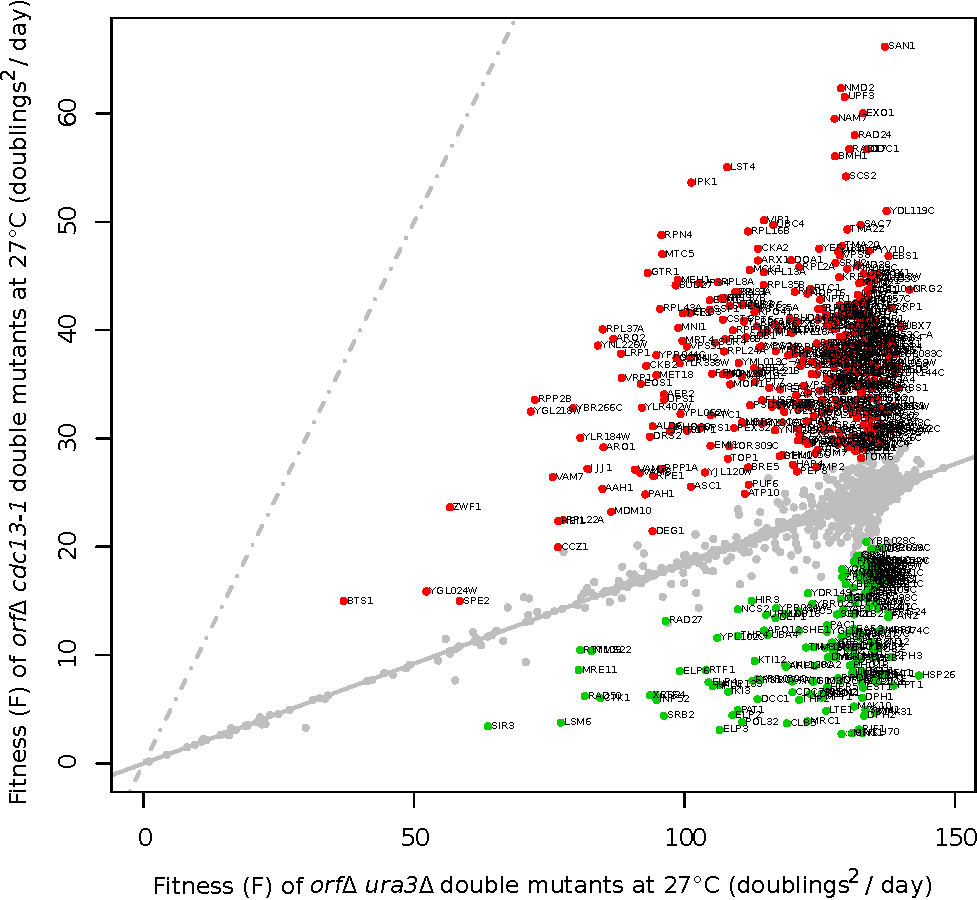
\includegraphics[height=0.8\textheight]{figs/IHM}}
}

\frame{
\frametitle{Joint modelling of growth curves and genetic interaction}
\begin{itemize}
\item We can integrate together the hierarchical growth curve model
  and the genetic interaction model into a combined joint model
\item This has usual advantages of properly borrowing strength, proper
  propagation of uncertainty, etc.
\item Also very convenient to avoid requiring a scalar measure of
  ``fitness''
\item If $y_{clmn}$ is the colony size at time point $n$ in repeat $m$
  of gene $l$ in condition $c$, then
\begin{align*}
y_{clmn} &\sim N(\hat{y}_{clmn},1/\nu_{cl}) \\
\hat{y}_{clmn} &= X(t_{clmn};K_{clm},r_{clm},P) \\
\log K_{clm} &\sim
N(\alpha_c+K_l^o+\delta_l\gamma_{cl},1/\tau_{cl}^K)\\
\log r_{clm} &\sim N(\beta_{c}+r_l^o+\delta_l\omega_{cl},1/\tau_{cl}^r)
\end{align*}
\end{itemize}
}

\frame{
\frametitle{Joint model}
\centerline{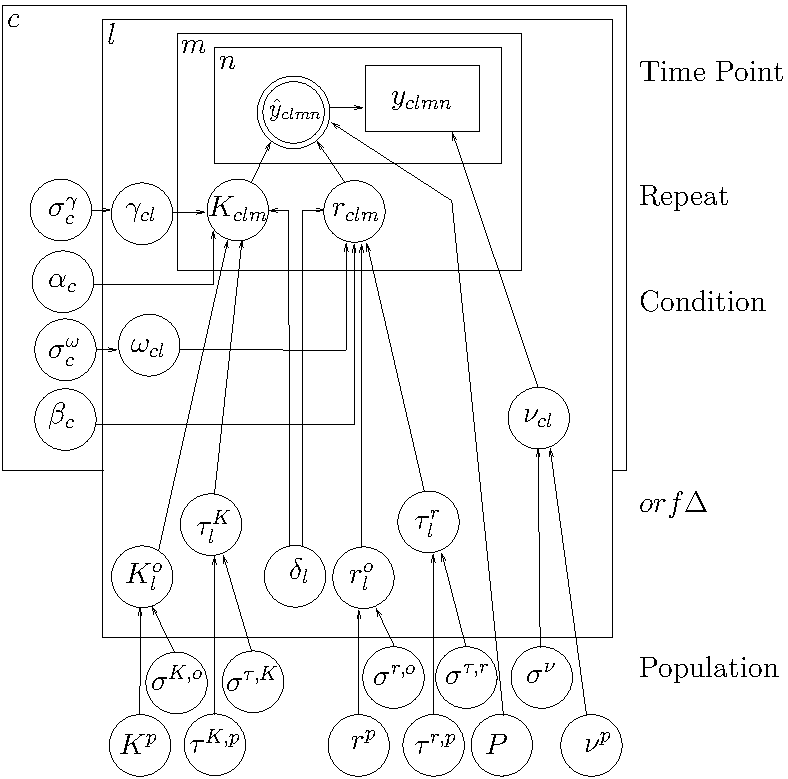
\includegraphics[height=0.8\textheight]{figs/DAG3}}
}

\frame{
\frametitle{Joint model results}
\centerline{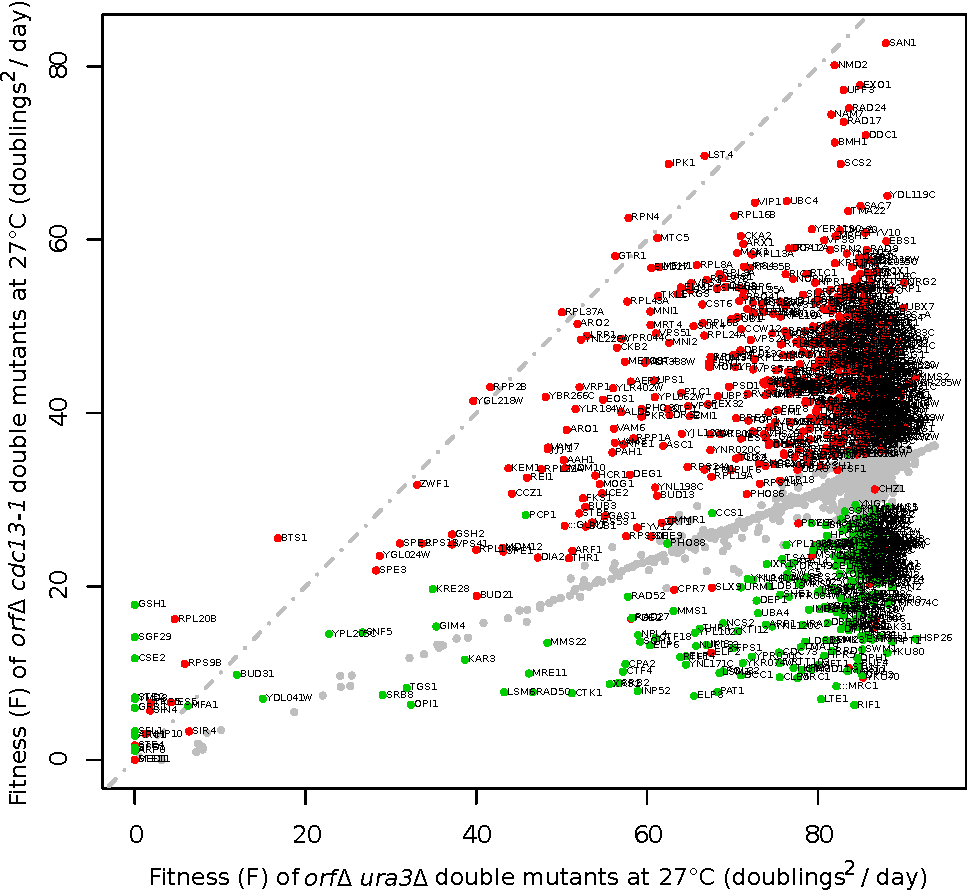
\includegraphics[height=0.8\textheight]{figs/JHM}}
}

\subsection{MiniQFA}

\frame{
\frametitle{MiniQFA}
Not just a single query, but an ``all-by-all" experiment for a (small) subset of the genome
  \begin{itemize}
  \item We have run an experiment with 150 gene knockouts (in both wt and cdc13-1 backgrounds) on a single plate, using each in turn as the query mutation, to map out the full set of pairwise interactions for the subset
  \item Requires an extension and some modification of the previous hierarchical models
  \item Enables an in depth study of the prevelance of genetic interaction, and will allow consideration of alternative notions of genetic interaction and epistasis, which could distinguish between ``direct" and ``indirect" interactions
  \end{itemize}
%\end{itemize}
}

\frame{
\frametitle{MiniQFA model}
\begin{itemize}
\item Initial modelling approach based on two stages
\item Interaction model:
\begin{align*}
F_{ll'm} &\sim N(\hat{F}_{ll'm},1/\nu)\\
\log \hat{F}_{ll'm} &= \mu + Z_l + Z_{l'} + \delta_{ll'}\gamma_{ll'} \\
\delta_{ll'} &\sim \text{Bern}(p)
\end{align*}
\item A version assuming symmetry (eg. $\delta_{ll'}=\delta_{l'l}$, and similar for $\gamma_{ll'}$), and another which doesn't, another with $t$ errors, ...
\item Using preliminary data, only around 10\% of the $\binom{150}{2}\simeq 11$k potential interactions are being selected
\item Starting to think about implementation of the ``direct" versus ``indirect" model...
\end{itemize}
}

\frame{
\frametitle{Preliminary MiniQFA results (cdc13-1 at 27C)}
\centerline{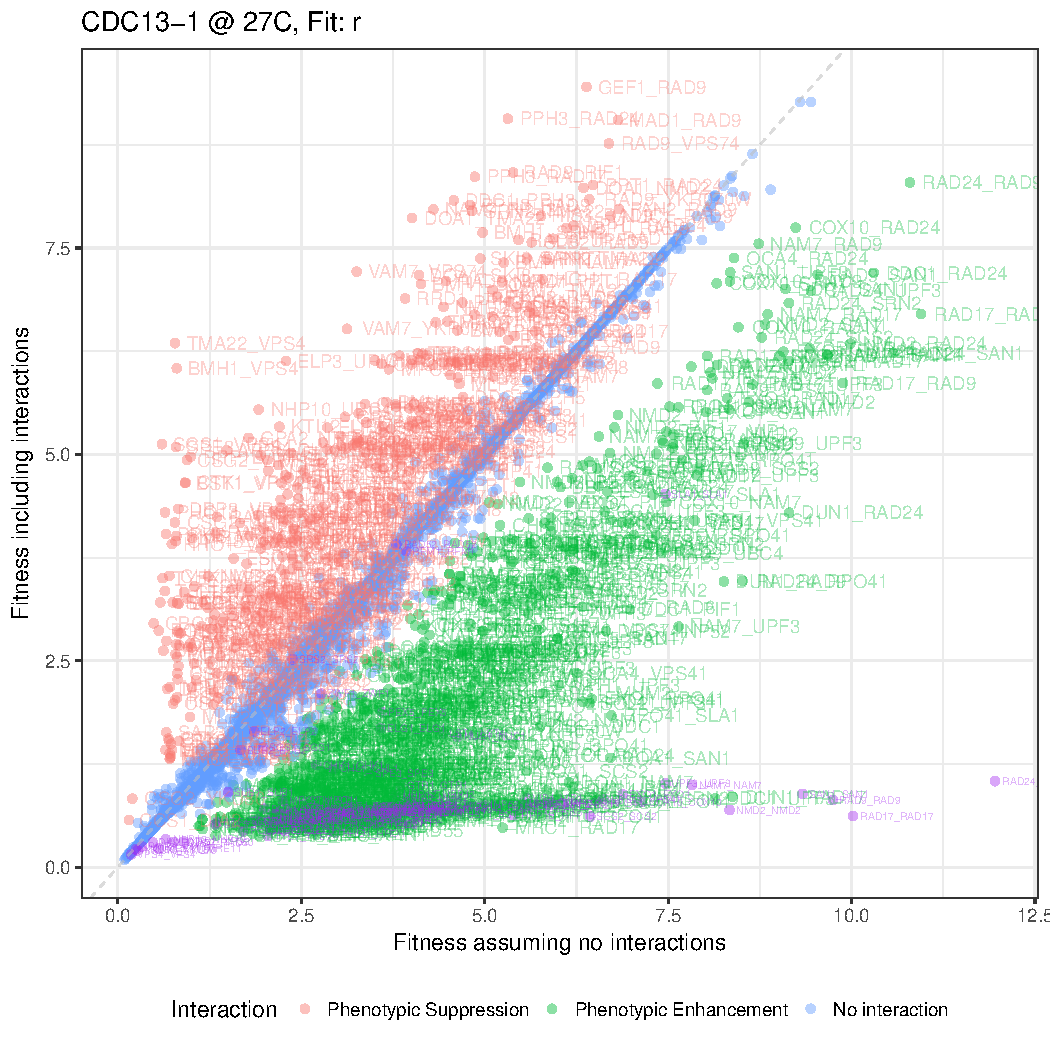
\includegraphics[height=0.9\textheight]{figs/mQFA_GISplot_FitCDC13D127}}
}

\frame{
\frametitle{All double deletions}
\centerline{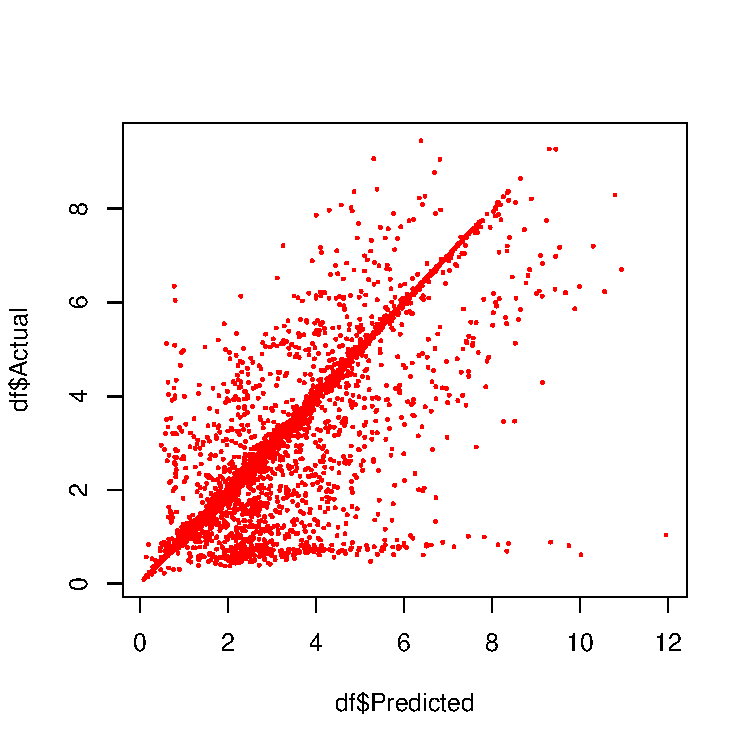
\includegraphics[height=0.9\textheight]{figs/mqfa-all}}
}

\frame{
\frametitle{Only the interacting double deletions}
\centerline{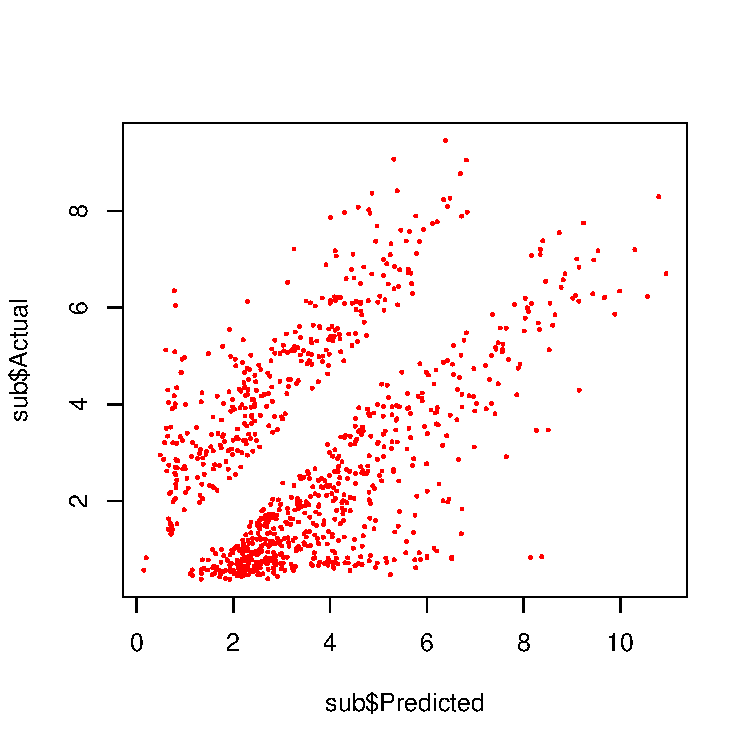
\includegraphics[height=0.9\textheight]{figs/mqfa-int}}
}

\frame{
\frametitle{Graph of pairwise interactions}
\centerline{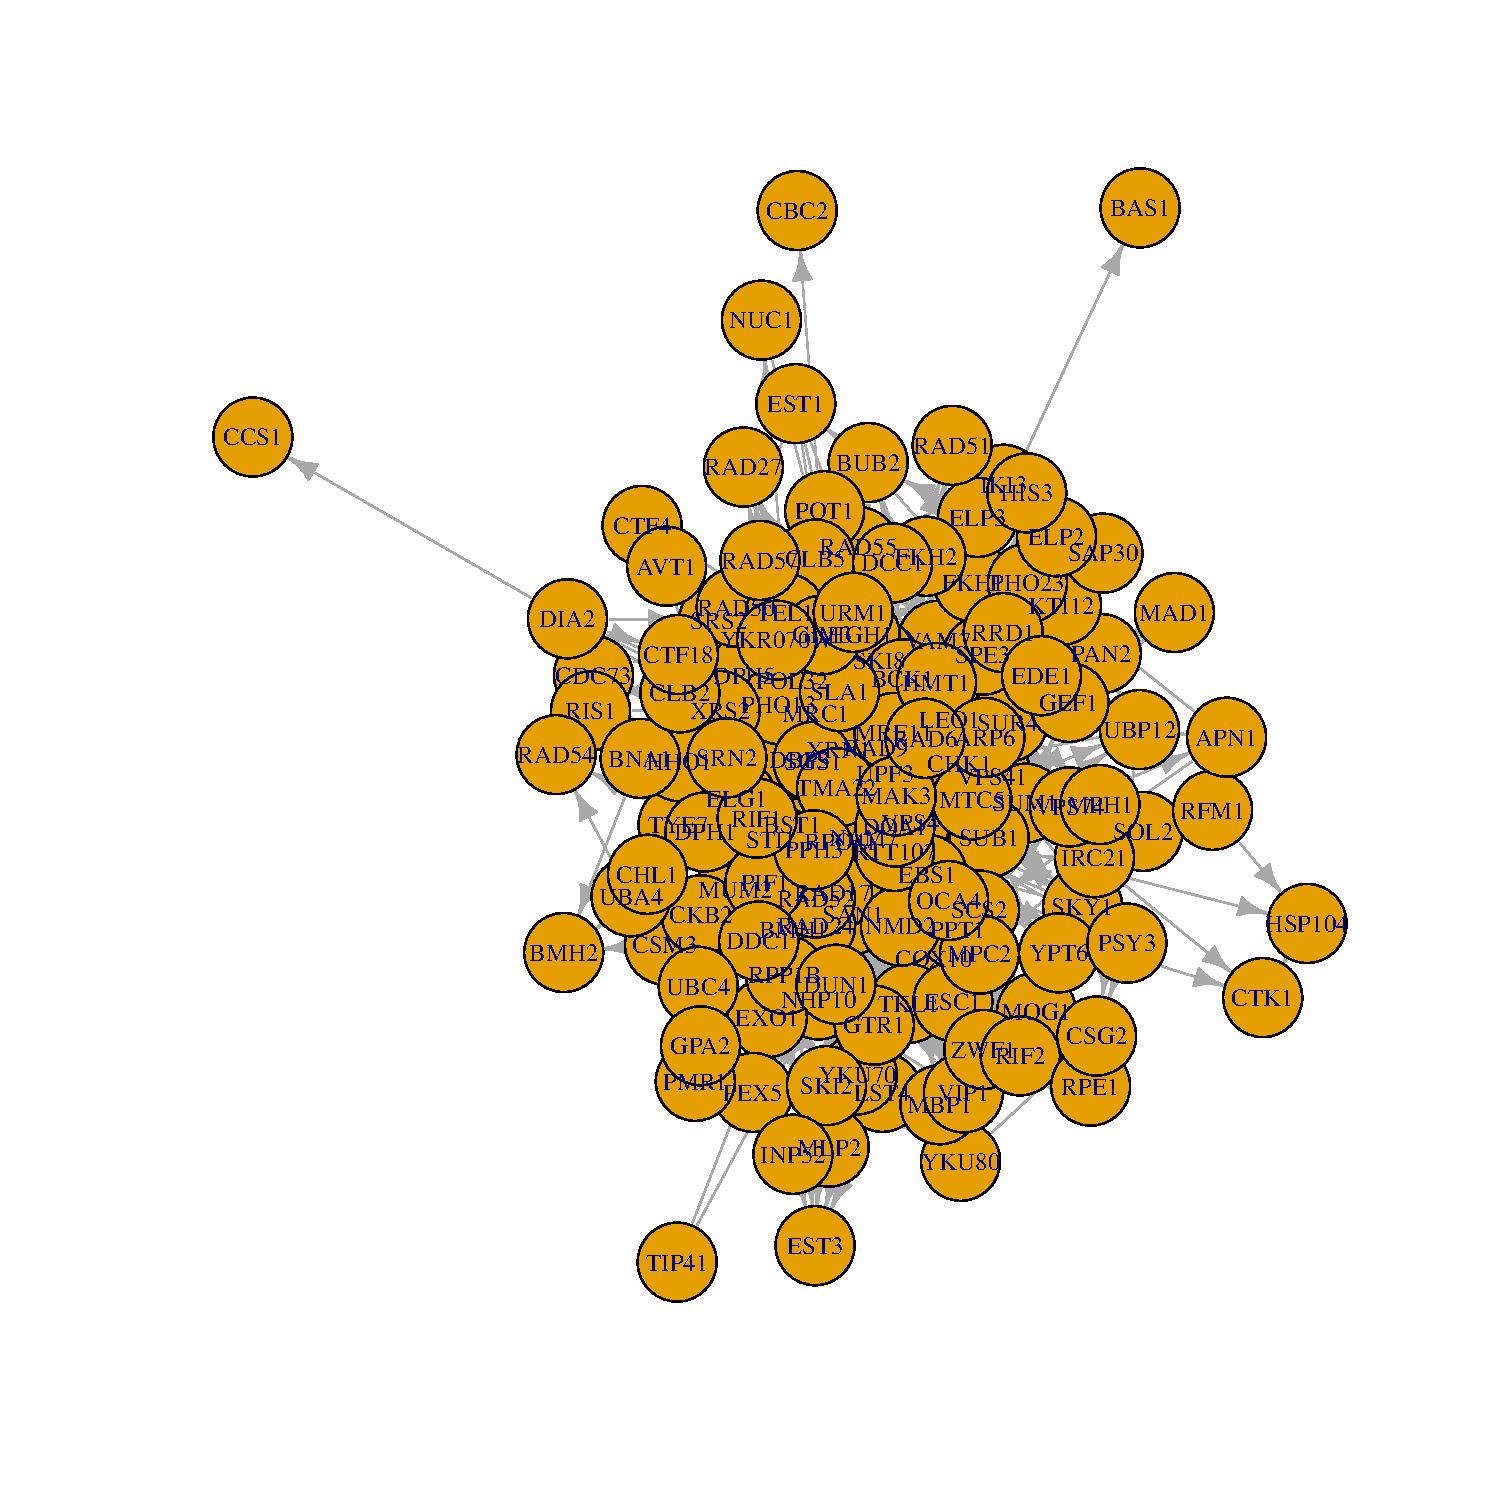
\includegraphics[height=0.9\textheight]{figs/mqfa-dag}}
}

\frame{
\frametitle{Circle layout}
\centerline{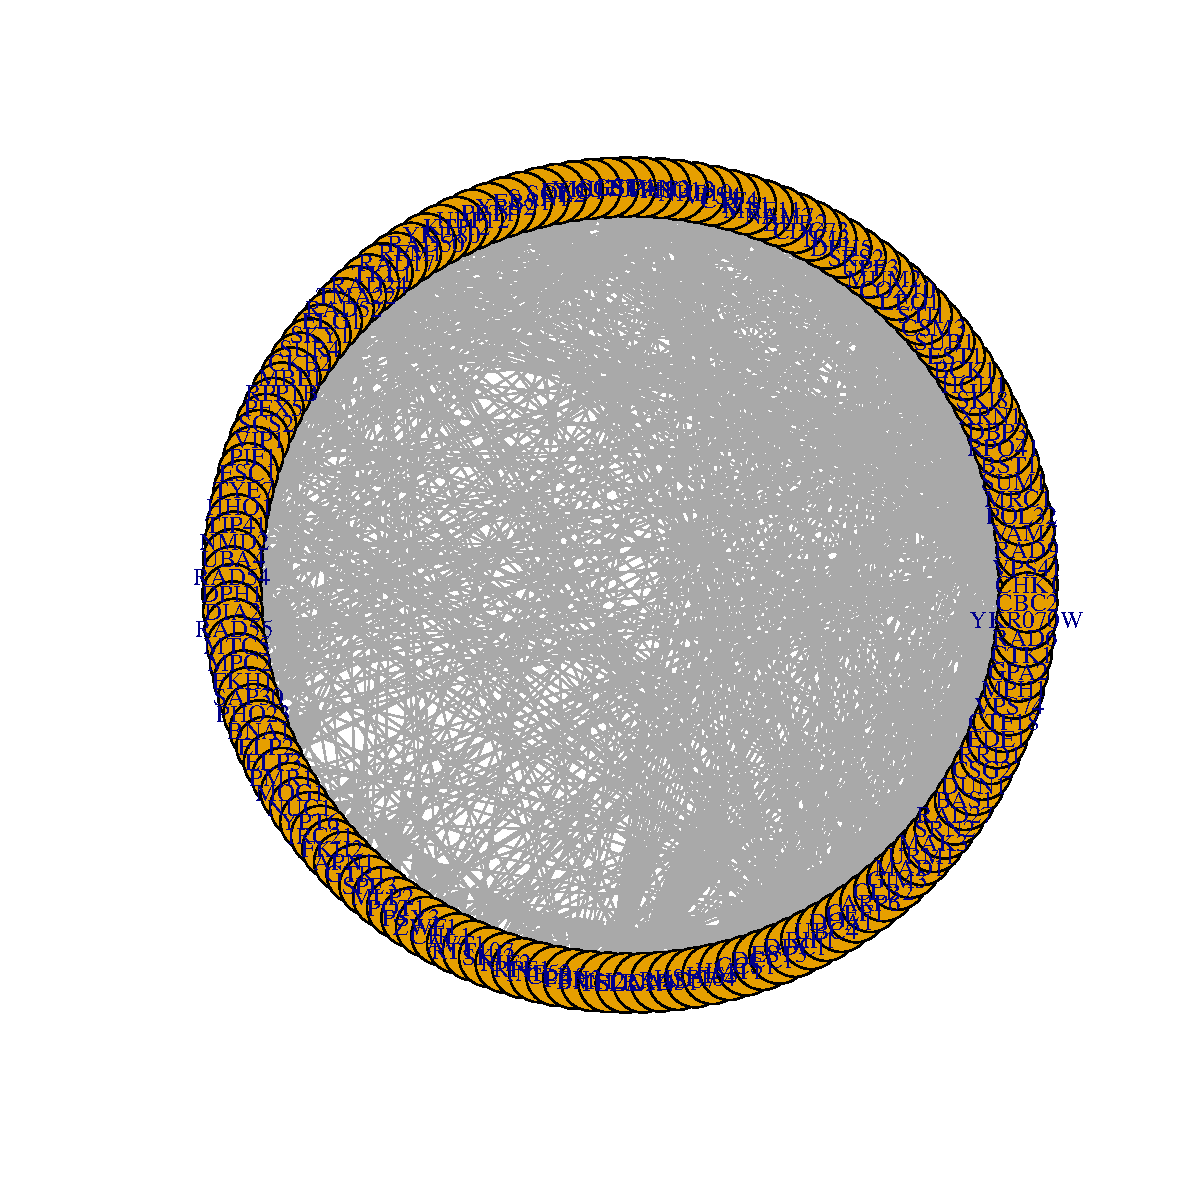
\includegraphics[height=0.9\textheight]{figs/mqfa-circ}}
}

\frame{
\frametitle{Adjacency matrix}
\centerline{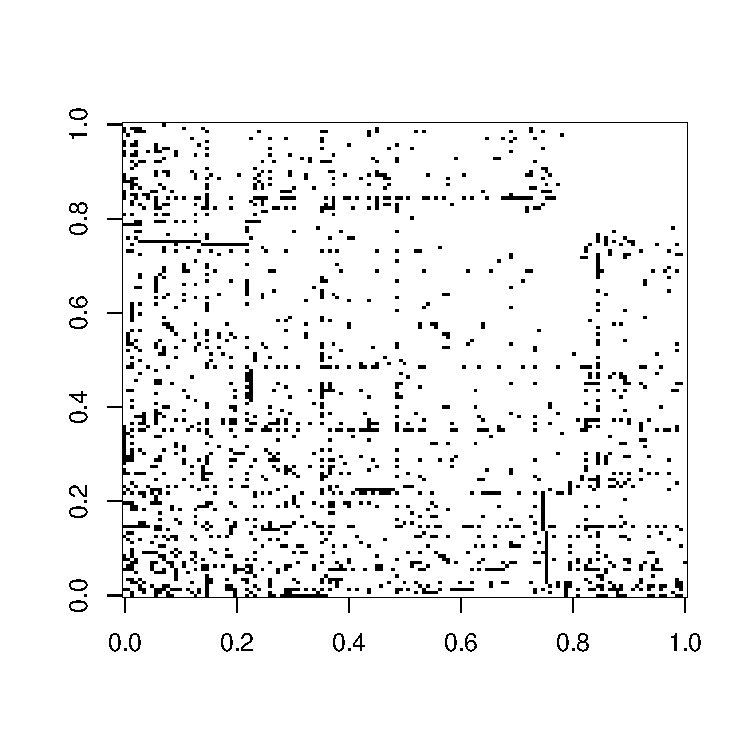
\includegraphics[height=0.9\textheight]{figs/mqfa-adj}}
}

\frame{
\frametitle{Adjacency matrix (``fast greedy'' graph clustering)}
\centerline{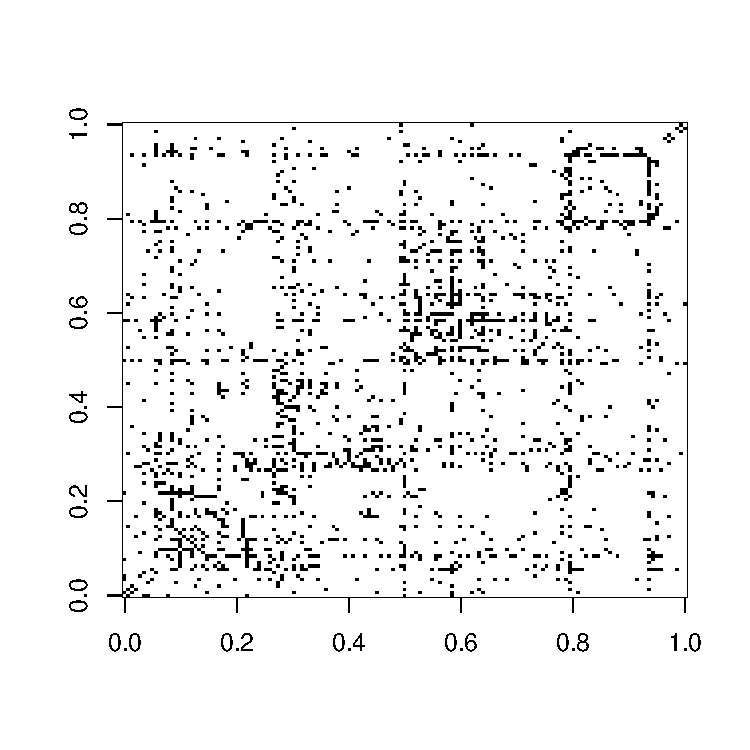
\includegraphics[height=0.9\textheight]{figs/mqfa-adj-fg}}
}

\frame{
\frametitle{Interaction graph (``fast greedy'' graph clustering)}
\centerline{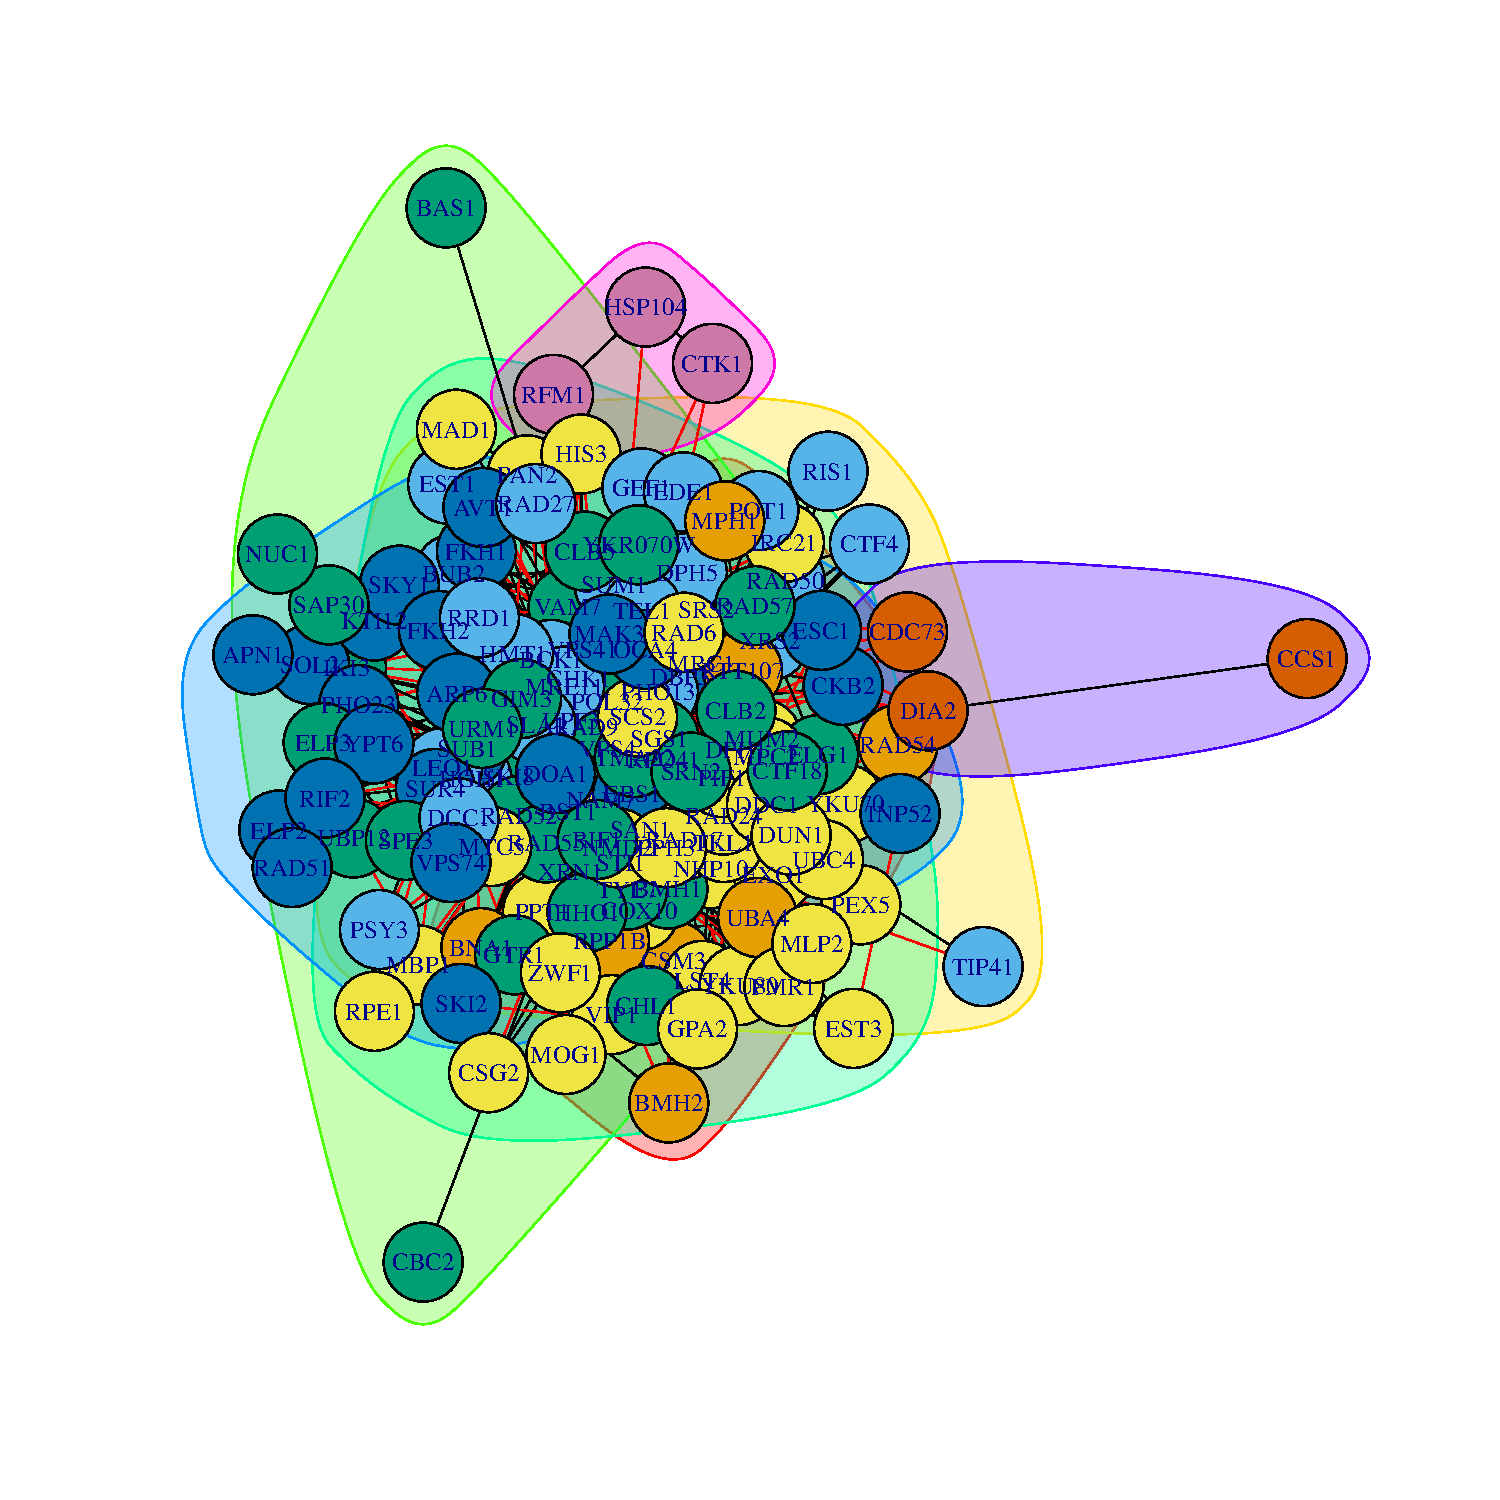
\includegraphics[height=0.9\textheight]{figs/mqfa-ug-fg}}
}

\frame{
\frametitle{Adjacency matrix (``spin--glass'' graph clustering)}
\centerline{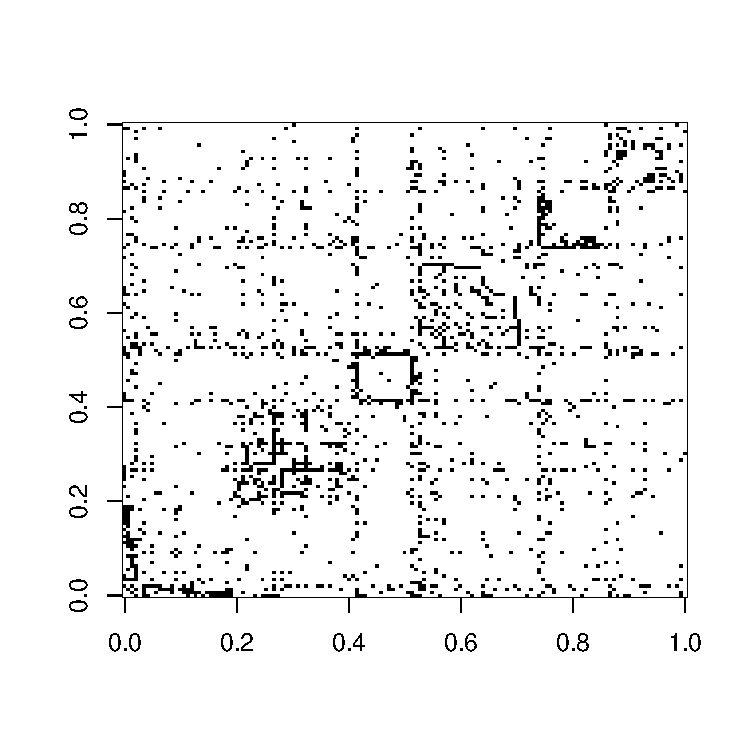
\includegraphics[height=0.9\textheight]{figs/mqfa-adj-sg}}
}

\frame{
\frametitle{Interaction graph (``spin--glass'' graph clustering)}
\centerline{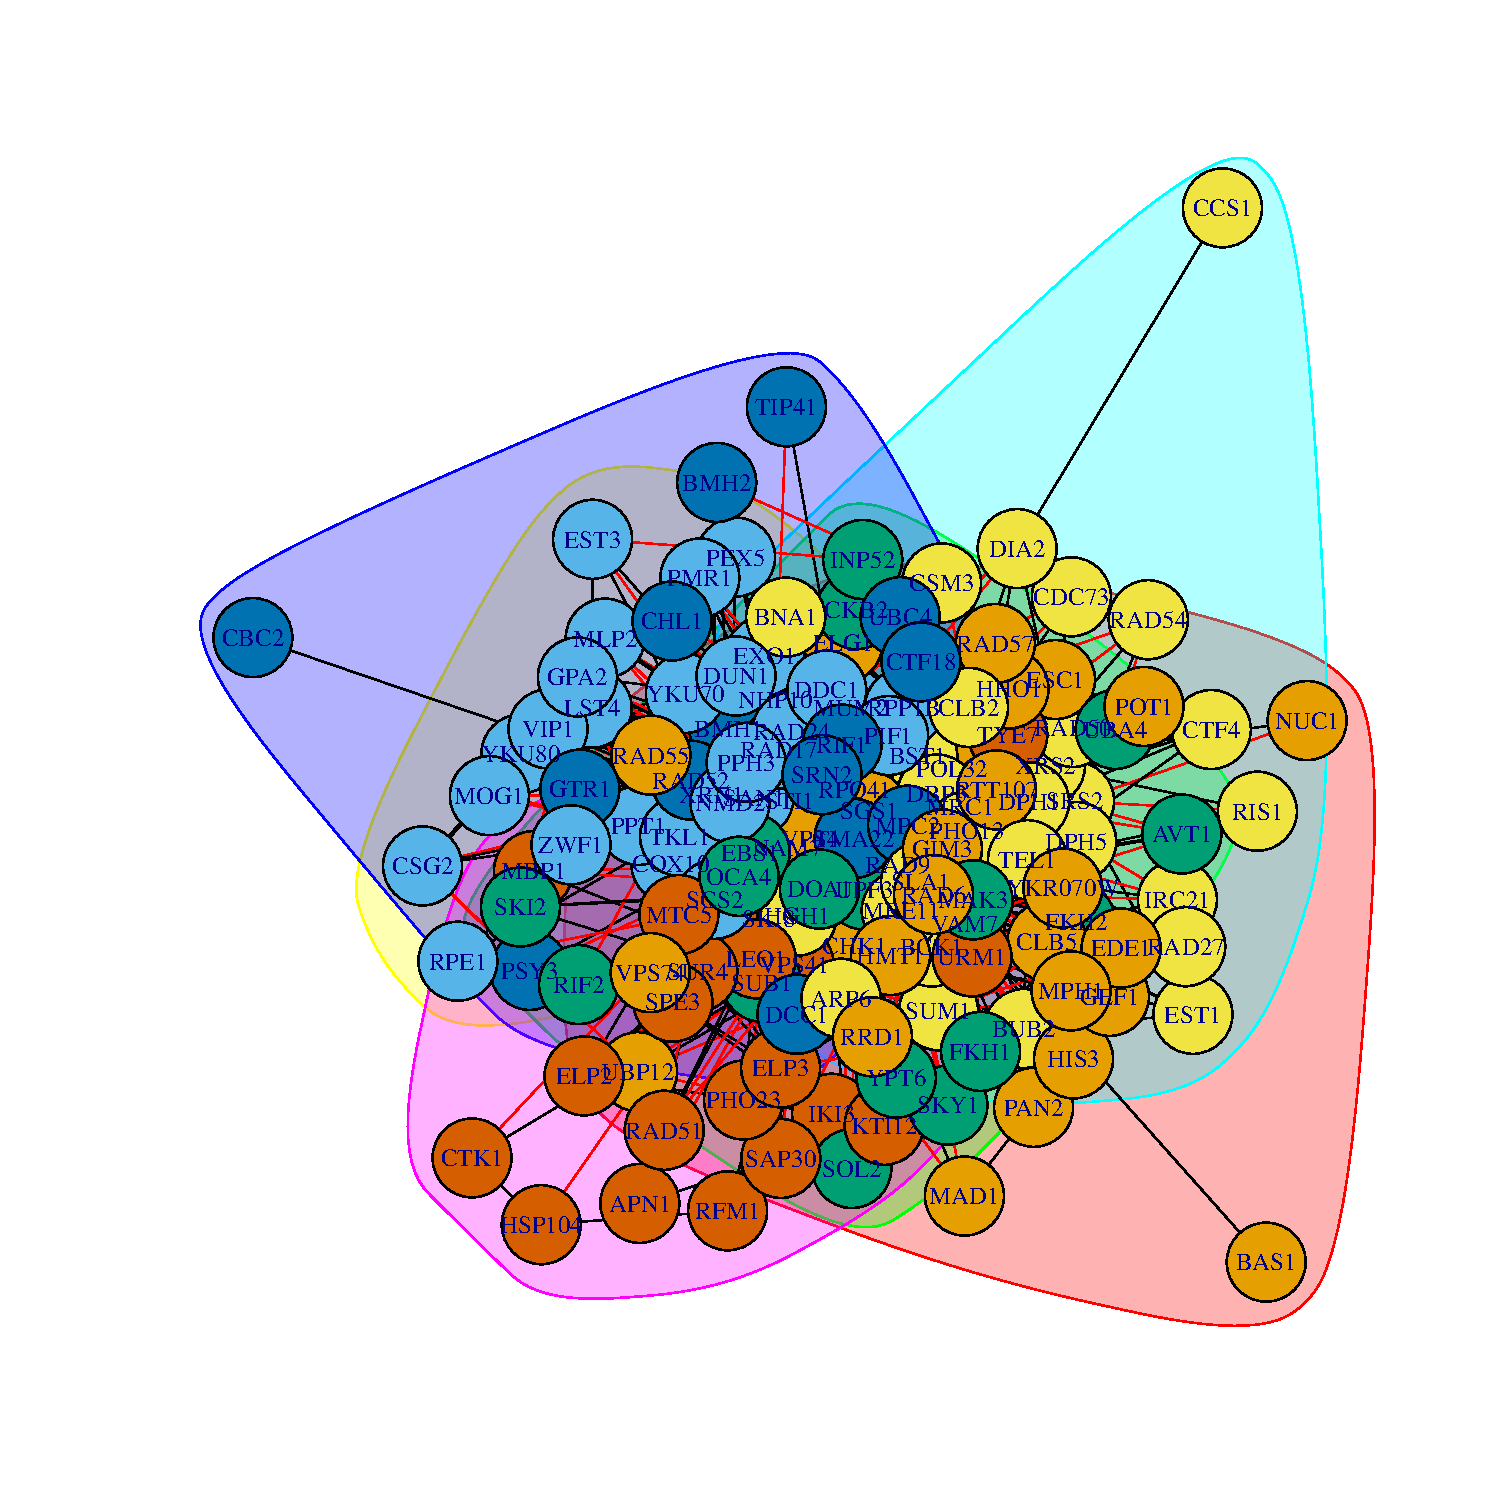
\includegraphics[height=0.9\textheight]{figs/mqfa-ug-sg}}
}

\section{Summary and conclusions}
%\section{Computational issues}

\begin{comment}
  
% \subsection{``Big data'' issues}

\frame{
\frametitle{``Big data'' issues}
\begin{itemize}
\item Understanding \alert{conflict} between model and data in big data contexts --- does more data demand \alert{more complex models}?
\item Model \alert{simplifications} and improvements to MCMC (linear Gaussian block updates and proposals, ``INLA proposals'', 2-block proposals, reparameterisations, GVS, etc.)
\item Basic \alert{parallelisation} strategies (parallel chains, parallellelised single chain)
\item Investigation of \alert{data parallel} strategies (consensus Monte Carlo, etc.)
\item Novel representations, interpretations and implementations of Bayesian hierarchical models using ideas from \alert{probabilistic programming} and strongly typed \alert{functional programming languages} (Scala, Haskell, Eta, OCaml, ...)
\end{itemize}
}

\end{comment}

\subsection{Summary}

\frame{
\frametitle{Summary}
\begin{itemize}
\item Modern bioscience is generating large, complex data sets which
  require \alert{sophisticated modelling} in order to answer questions of
  scientific interest
\item Big data forces \alert{trade-offs} between statistical accuracy and
  computational tractability
\item \alert{Stochastic dynamic models} are much more flexible than deterministic
  models, but come at a computational cost --- the LNA can
  sometimes represent an excellent compromise
\item Notions of \alert{genetic interaction} translate directly to statistical
  models of interaction
\item Big hierarchical \alert{variable selection} models are useful in genomics, but can be computationally challenging
\end{itemize}
}


\begin{comment}
  
\frame{
\frametitle{Funding acknowledgements}
Major funders of this work:
\begin{itemize}
\item BBSRC (RCUK)
\item MRC (RCUK)
\item Wellcome Trust
\item Cancer Research UK
\end{itemize}
}

\end{comment}

\subsection{References}

\frame{
\frametitle{References}
\begin{thebibliography}{}

%\small
\scriptsize

%\bibitem[\protect\citeauthoryear{blah}{blah}{2006}]{blah}
%Boys, R.~J., D.~J. Wilkinson and T.~B.~L. Kirkwood (2008)  Bayesian
%inference for a discretely observed stochastic kinetic model. {\em
%Statistics and Computing,\/}~\textbf{18}(2), 125--135.

%\bibitem[\protect\citeauthoryear{Golightly and Wilkinson}{Golightly and
%  Wilkinson}{2006}]{GoliWilk06}
%Golightly, A. and D.~J. Wilkinson (2006).
% Bayesian sequential inference for stochastic kinetic biochemical
%  network models. {\em Journal of Computational Biology.\/}~{\em
%13\/}(3), 838--851.

\bibitem[\protect\citeauthoryear{blah}{blah}{2011}]{blah}
Addinall, S. G. et al (2011)
\alert{\href{http://dx.doi.org/10.1371/journal.pgen.1001362}{Quantitative
    fitness analysis shows that NMD proteins and many other protein
    complexes suppress or enhance distinct telomere cap
    defects}}. {\em PLoS Genetics\/}, \textbf{7}:e1001362.

%\bibitem[\protect\citeauthoryear{blah}{blah}{2011}]{blah}
%Golightly, A. and D.~J. Wilkinson (2011)
%\alert{\href{http://rsfs.royalsocietypublishing.org/content/early/2011/09/27/rsfs.2011.0047.abstract}{Bayesian parameter inference for stochastic biochemical network models
%using particle MCMC}}. {\em Interface Focus\/}, \textbf{1}(6):807--820.

%\bibitem[\protect\citeauthoryear{blah}{blah}{2006}]{blah}
%Golightly, A. and D.~J. Wilkinson (2008)
%\alert{Bayesian inference for nonlinear multivariate diffusion models
%observed with error}. {\em Computational Statistics and Data
%Analysis,\/}~\textbf{52}(3), 1674--1693.

\bibitem{blah}
Heydari, J. J. et al (2016)
\alert{Bayesian hierarchical modelling for inferring genetic interactions in
yeast}, {\em Journal of the Royal Statistical Society, Series C}, \textbf{65}(3):367--393.

%\bibitem{blah}
%Heydari, J. J. et al (2014)
%\alert{Fast Bayesian parameter estimation for stochastic logistic growth models}, {\em BioSystems}, \textbf{122}:55-72.

%\bibitem{blah}
%Lawless, C., Wilkinson, D. J., Addinall, S. G., Lydall, D. A. (2010)
%\alert{Colonyzer: automated quantification of characteristics of
%  microorganism colonies growing on solid agar}, {\em BMC Bioinformatics}, \textbf{11}:287. 

%\bibitem[\protect\citeauthoryear{blah}{blah}{2011}]{blah}
%Lei, G., Boys, R.~J., Gillespie, C.~S., Greenall, A.~J., Wilkinson, D.~J. (2011)
%\alert{\href{http://dx.doi.org/10.4172/2155-6180.1000127}{Bayesian
%    inference for sparse VAR(1) models, with application to time
%    course microarray data}}. {\em Journal of Biometrics and Biostatistics\/}, \textbf{2}:127.

%\bibitem[\protect\citeauthoryear{blah}{blah}{2012}]{blah}
%Weile, J., James, K., Hallinan, J., Cockell, S. J., Lord, P., Wipat, A., Wilkinson, D. J. (2012)
%\alert{\href{http://dx.doi.org/10.1093/bioinformatics/bts154}{Bayesian integration of networks without gold standards}}. {\em Bioinformatics\/}, \textbf{28}:1495--1500.



%\bibitem[\protect\citeauthoryear{blah}{blah}{2009}]{blah}Henderson,
%D. A., Boys, R. J., Krishnan, K. J., Lawless, C., Wilkinson,
%D. J. (2009) Bayesian emulation and calibration of a stochastic
%computer model of mitochondrial DNA deletions in substantia nigra
%neurons, {\em Journal of the American Statistical
%Association.\/}~\textbf{104}(485):76-87. 

%\bibitem[\protect\citeauthoryear{blah}{blah}{2009}]{blah}Henderson,
%D. A., Boys, R. J., Proctor, C. J., Wilkinson, D. J. (2010) \alert{Linking systems biology models to data: a stochastic kinetic model of p53 oscillations\/}, A. O'Hagan and M. West (eds.) Handbook of Applied Bayesian Analysis, Oxford University Press.

\bibitem[\protect\citeauthoryear{blah}{blah}{2009}]{blah}Wilkinson,
D. J. (2009) \alert{\href{http://dx.doi.org/10.1038/nrg2509}{Stochastic modelling for quantitative description of
heterogeneous biological systems}}, {\em Nature Reviews Genetics.\/}~\textbf{10}(2):122-133.

%\bibitem[\protect\citeauthoryear{blah}{blah}{2010}]{blah}Wilkinson,
%  D. J. (2010) \alert{\href{http://www.mas.ncl.ac.uk/~ndjw1/docs/Wilkinson10.pdf}{Parameter inference for stochastic kinetic models of
%  bacterial gene regulation: a Bayesian approach to systems biology}}
%  (with discussion), in J.-M. Bernardo et al (eds) {\em Bayesian
%    Statistics 9,\/} OUP, pp.679--706.

\beamertemplatebookbibitems

%\bibitem[\protect\citeauthoryear{Wilkinson}{Wilkinson}{2006}]{Wilkinson06}
%Wilkinson, D.~J. (2006)
% {\em Stochastic Modelling for Systems Biology}.
% Chapman \& Hall/CRC Press. \alert{(second edition in press)}

\bibitem[\protect\citeauthoryear{Wilkinson}{Wilkinson}{2011}]{Wilkinson11}
Wilkinson, D.~J. (2018)
 {\em \alert{\href{http://github.com/darrenjw/smfsb}{Stochastic Modelling for Systems Biology, third edition}}}.
 Chapman \& Hall/CRC Press.

\end{thebibliography}

\medskip

%\centerline{Me: \large{\alert{\url{tinyurl.com/darrenjw}}}}

%\begin{block}{Contact details...}
%email: \url{darren.wilkinson@ncl.ac.uk} \\
%%www: \url{http://www.staff.ncl.ac.uk/d.j.wilkinson/}
%www: \url{tinyurl.com/darrenjw}
%\end{block}

%\medskip

%\centerline{Draft manuscript: {\large\alert{\url{tinyurl.com/y3jkmlp}}}}


}




\end{document}
